% Options for packages loaded elsewhere
\PassOptionsToPackage{unicode}{hyperref}
\PassOptionsToPackage{hyphens}{url}
\PassOptionsToPackage{dvipsnames,svgnames,x11names}{xcolor}
%
\documentclass[
  letterpaper,
  DIV=11,
  numbers=noendperiod]{scrartcl}

\usepackage{amsmath,amssymb}
\usepackage{iftex}
\ifPDFTeX
  \usepackage[T1]{fontenc}
  \usepackage[utf8]{inputenc}
  \usepackage{textcomp} % provide euro and other symbols
\else % if luatex or xetex
  \usepackage{unicode-math}
  \defaultfontfeatures{Scale=MatchLowercase}
  \defaultfontfeatures[\rmfamily]{Ligatures=TeX,Scale=1}
\fi
\usepackage{lmodern}
\ifPDFTeX\else  
    % xetex/luatex font selection
\fi
% Use upquote if available, for straight quotes in verbatim environments
\IfFileExists{upquote.sty}{\usepackage{upquote}}{}
\IfFileExists{microtype.sty}{% use microtype if available
  \usepackage[]{microtype}
  \UseMicrotypeSet[protrusion]{basicmath} % disable protrusion for tt fonts
}{}
\makeatletter
\@ifundefined{KOMAClassName}{% if non-KOMA class
  \IfFileExists{parskip.sty}{%
    \usepackage{parskip}
  }{% else
    \setlength{\parindent}{0pt}
    \setlength{\parskip}{6pt plus 2pt minus 1pt}}
}{% if KOMA class
  \KOMAoptions{parskip=half}}
\makeatother
\usepackage{xcolor}
\setlength{\emergencystretch}{3em} % prevent overfull lines
\setcounter{secnumdepth}{-\maxdimen} % remove section numbering
% Make \paragraph and \subparagraph free-standing
\ifx\paragraph\undefined\else
  \let\oldparagraph\paragraph
  \renewcommand{\paragraph}[1]{\oldparagraph{#1}\mbox{}}
\fi
\ifx\subparagraph\undefined\else
  \let\oldsubparagraph\subparagraph
  \renewcommand{\subparagraph}[1]{\oldsubparagraph{#1}\mbox{}}
\fi

\usepackage{color}
\usepackage{fancyvrb}
\newcommand{\VerbBar}{|}
\newcommand{\VERB}{\Verb[commandchars=\\\{\}]}
\DefineVerbatimEnvironment{Highlighting}{Verbatim}{commandchars=\\\{\}}
% Add ',fontsize=\small' for more characters per line
\usepackage{framed}
\definecolor{shadecolor}{RGB}{241,243,245}
\newenvironment{Shaded}{\begin{snugshade}}{\end{snugshade}}
\newcommand{\AlertTok}[1]{\textcolor[rgb]{0.68,0.00,0.00}{#1}}
\newcommand{\AnnotationTok}[1]{\textcolor[rgb]{0.37,0.37,0.37}{#1}}
\newcommand{\AttributeTok}[1]{\textcolor[rgb]{0.40,0.45,0.13}{#1}}
\newcommand{\BaseNTok}[1]{\textcolor[rgb]{0.68,0.00,0.00}{#1}}
\newcommand{\BuiltInTok}[1]{\textcolor[rgb]{0.00,0.23,0.31}{#1}}
\newcommand{\CharTok}[1]{\textcolor[rgb]{0.13,0.47,0.30}{#1}}
\newcommand{\CommentTok}[1]{\textcolor[rgb]{0.37,0.37,0.37}{#1}}
\newcommand{\CommentVarTok}[1]{\textcolor[rgb]{0.37,0.37,0.37}{\textit{#1}}}
\newcommand{\ConstantTok}[1]{\textcolor[rgb]{0.56,0.35,0.01}{#1}}
\newcommand{\ControlFlowTok}[1]{\textcolor[rgb]{0.00,0.23,0.31}{#1}}
\newcommand{\DataTypeTok}[1]{\textcolor[rgb]{0.68,0.00,0.00}{#1}}
\newcommand{\DecValTok}[1]{\textcolor[rgb]{0.68,0.00,0.00}{#1}}
\newcommand{\DocumentationTok}[1]{\textcolor[rgb]{0.37,0.37,0.37}{\textit{#1}}}
\newcommand{\ErrorTok}[1]{\textcolor[rgb]{0.68,0.00,0.00}{#1}}
\newcommand{\ExtensionTok}[1]{\textcolor[rgb]{0.00,0.23,0.31}{#1}}
\newcommand{\FloatTok}[1]{\textcolor[rgb]{0.68,0.00,0.00}{#1}}
\newcommand{\FunctionTok}[1]{\textcolor[rgb]{0.28,0.35,0.67}{#1}}
\newcommand{\ImportTok}[1]{\textcolor[rgb]{0.00,0.46,0.62}{#1}}
\newcommand{\InformationTok}[1]{\textcolor[rgb]{0.37,0.37,0.37}{#1}}
\newcommand{\KeywordTok}[1]{\textcolor[rgb]{0.00,0.23,0.31}{#1}}
\newcommand{\NormalTok}[1]{\textcolor[rgb]{0.00,0.23,0.31}{#1}}
\newcommand{\OperatorTok}[1]{\textcolor[rgb]{0.37,0.37,0.37}{#1}}
\newcommand{\OtherTok}[1]{\textcolor[rgb]{0.00,0.23,0.31}{#1}}
\newcommand{\PreprocessorTok}[1]{\textcolor[rgb]{0.68,0.00,0.00}{#1}}
\newcommand{\RegionMarkerTok}[1]{\textcolor[rgb]{0.00,0.23,0.31}{#1}}
\newcommand{\SpecialCharTok}[1]{\textcolor[rgb]{0.37,0.37,0.37}{#1}}
\newcommand{\SpecialStringTok}[1]{\textcolor[rgb]{0.13,0.47,0.30}{#1}}
\newcommand{\StringTok}[1]{\textcolor[rgb]{0.13,0.47,0.30}{#1}}
\newcommand{\VariableTok}[1]{\textcolor[rgb]{0.07,0.07,0.07}{#1}}
\newcommand{\VerbatimStringTok}[1]{\textcolor[rgb]{0.13,0.47,0.30}{#1}}
\newcommand{\WarningTok}[1]{\textcolor[rgb]{0.37,0.37,0.37}{\textit{#1}}}

\providecommand{\tightlist}{%
  \setlength{\itemsep}{0pt}\setlength{\parskip}{0pt}}\usepackage{longtable,booktabs,array}
\usepackage{calc} % for calculating minipage widths
% Correct order of tables after \paragraph or \subparagraph
\usepackage{etoolbox}
\makeatletter
\patchcmd\longtable{\par}{\if@noskipsec\mbox{}\fi\par}{}{}
\makeatother
% Allow footnotes in longtable head/foot
\IfFileExists{footnotehyper.sty}{\usepackage{footnotehyper}}{\usepackage{footnote}}
\makesavenoteenv{longtable}
\usepackage{graphicx}
\makeatletter
\def\maxwidth{\ifdim\Gin@nat@width>\linewidth\linewidth\else\Gin@nat@width\fi}
\def\maxheight{\ifdim\Gin@nat@height>\textheight\textheight\else\Gin@nat@height\fi}
\makeatother
% Scale images if necessary, so that they will not overflow the page
% margins by default, and it is still possible to overwrite the defaults
% using explicit options in \includegraphics[width, height, ...]{}
\setkeys{Gin}{width=\maxwidth,height=\maxheight,keepaspectratio}
% Set default figure placement to htbp
\makeatletter
\def\fps@figure{htbp}
\makeatother

\KOMAoption{captions}{tableheading}
\makeatletter
\@ifpackageloaded{tcolorbox}{}{\usepackage[skins,breakable]{tcolorbox}}
\@ifpackageloaded{fontawesome5}{}{\usepackage{fontawesome5}}
\definecolor{quarto-callout-color}{HTML}{909090}
\definecolor{quarto-callout-note-color}{HTML}{0758E5}
\definecolor{quarto-callout-important-color}{HTML}{CC1914}
\definecolor{quarto-callout-warning-color}{HTML}{EB9113}
\definecolor{quarto-callout-tip-color}{HTML}{00A047}
\definecolor{quarto-callout-caution-color}{HTML}{FC5300}
\definecolor{quarto-callout-color-frame}{HTML}{acacac}
\definecolor{quarto-callout-note-color-frame}{HTML}{4582ec}
\definecolor{quarto-callout-important-color-frame}{HTML}{d9534f}
\definecolor{quarto-callout-warning-color-frame}{HTML}{f0ad4e}
\definecolor{quarto-callout-tip-color-frame}{HTML}{02b875}
\definecolor{quarto-callout-caution-color-frame}{HTML}{fd7e14}
\makeatother
\makeatletter
\makeatother
\makeatletter
\makeatother
\makeatletter
\@ifpackageloaded{caption}{}{\usepackage{caption}}
\AtBeginDocument{%
\ifdefined\contentsname
  \renewcommand*\contentsname{Table of contents}
\else
  \newcommand\contentsname{Table of contents}
\fi
\ifdefined\listfigurename
  \renewcommand*\listfigurename{List of Figures}
\else
  \newcommand\listfigurename{List of Figures}
\fi
\ifdefined\listtablename
  \renewcommand*\listtablename{List of Tables}
\else
  \newcommand\listtablename{List of Tables}
\fi
\ifdefined\figurename
  \renewcommand*\figurename{Figure}
\else
  \newcommand\figurename{Figure}
\fi
\ifdefined\tablename
  \renewcommand*\tablename{Table}
\else
  \newcommand\tablename{Table}
\fi
}
\@ifpackageloaded{float}{}{\usepackage{float}}
\floatstyle{ruled}
\@ifundefined{c@chapter}{\newfloat{codelisting}{h}{lop}}{\newfloat{codelisting}{h}{lop}[chapter]}
\floatname{codelisting}{Listing}
\newcommand*\listoflistings{\listof{codelisting}{List of Listings}}
\makeatother
\makeatletter
\@ifpackageloaded{caption}{}{\usepackage{caption}}
\@ifpackageloaded{subcaption}{}{\usepackage{subcaption}}
\makeatother
\makeatletter
\@ifpackageloaded{tcolorbox}{}{\usepackage[skins,breakable]{tcolorbox}}
\makeatother
\makeatletter
\@ifundefined{shadecolor}{\definecolor{shadecolor}{rgb}{.97, .97, .97}}
\makeatother
\makeatletter
\makeatother
\makeatletter
\makeatother
\ifLuaTeX
  \usepackage{selnolig}  % disable illegal ligatures
\fi
\IfFileExists{bookmark.sty}{\usepackage{bookmark}}{\usepackage{hyperref}}
\IfFileExists{xurl.sty}{\usepackage{xurl}}{} % add URL line breaks if available
\urlstyle{same} % disable monospaced font for URLs
\hypersetup{
  pdftitle={Impact of Women's Education on Fertility Rates Botswana},
  pdfauthor={Kaushika Potluri},
  colorlinks=true,
  linkcolor={blue},
  filecolor={Maroon},
  citecolor={Blue},
  urlcolor={Blue},
  pdfcreator={LaTeX via pandoc}}

\title{Impact of Women's Education on Fertility Rates Botswana}
\author{Kaushika Potluri}
\date{2022-11-11}

\begin{document}
\maketitle
\ifdefined\Shaded\renewenvironment{Shaded}{\begin{tcolorbox}[enhanced, frame hidden, breakable, borderline west={3pt}{0pt}{shadecolor}, interior hidden, boxrule=0pt, sharp corners]}{\end{tcolorbox}}\fi

\hypertarget{introduction}{%
\section{Introduction}\label{introduction}}

The research question that I have been interested in is the impact of
education about sex and fertility for women and how that changes the
fertility rate.

Women's education raises the value of time spent working in the market
and, as a result, the opportunity cost of spending time to take care of
their child seems less. Across time and places, there is a clear
negative link between women's education and fertility, although its
meaning is ambiguous. Women's level of education may impact fertility
through its effects on children's health, the number of children
desired, and women's ability to give birth and understanding of various
birth control options. Each of these are influenced by local,
institutional, and national circumstances. Their relative importance may
fluctuate as a society develops economically. We analyse the
education--fertility relationship by using data on women from Botswana.
A realistic quantification of such a relationship can be problematic for
various reasons. First, factors such as motivation and ability are
associated with fertility and education but cannot be observed and as a
consequence cannot be included in the model.

The central research question of this project revolves around
understanding the intricate relationship between women's education and
fertility rates. It delves into how education about sex and fertility
for women influences their decisions regarding childbirth, ultimately
impacting the fertility rate.

\hypertarget{theoretical-framework}{%
\subsection{Theoretical Framework}\label{theoretical-framework}}

Women's education plays a crucial role in shaping their priorities and
opportunities. As women become more educated, they often prioritize
career and personal development, which can lead to delayed childbearing.
This phenomenon is well-documented globally, showing a negative
correlation between women's education levels and fertility rates

Memory updated Sure, I can provide a fuller explanation and elaboration
on the content of your final project submission. Here's an expanded
version of the text with more detailed explanations and insights:

Final Project Submission: Impact of Women's Education on Fertility Rates
in Botswana Introduction The central research question of this project
revolves around understanding the intricate relationship between women's
education and fertility rates. It delves into how education about sex
and fertility for women influences their decisions regarding childbirth,
ultimately impacting the fertility rate.

Theoretical Framework Women's education plays a crucial role in shaping
their priorities and opportunities. As women become more educated, they
often prioritize career and personal development, which can lead to
delayed childbearing. This phenomenon is well-documented globally,
showing a negative correlation between women's education levels and
fertility rates.

\hypertarget{factors-influencing-fertility}{%
\subsubsection{Factors Influencing
Fertility}\label{factors-influencing-fertility}}

Several factors contribute to the complex dynamics of fertility rates
among women. These include:

Children's Health: Educated women are more likely to prioritize their
children's health, leading to smaller family sizes as they can allocate
more resources per child. Desired Number of Children: Education often
correlates with a desire for fewer children, as women focus on quality
over quantity. Birth Control Knowledge and Usage: Education empowers
women with knowledge about birth control options, leading to informed
family planning decisions. Socioeconomic Conditions: Local,
institutional, and national circumstances heavily influence fertility
rates, with economic development often leading to lower fertility rates.

\begin{tcolorbox}[enhanced jigsaw, leftrule=.75mm, breakable, opacityback=0, left=2mm, colback=white, bottomtitle=1mm, toptitle=1mm, arc=.35mm, colbacktitle=quarto-callout-tip-color!10!white, colframe=quarto-callout-tip-color-frame, rightrule=.15mm, opacitybacktitle=0.6, titlerule=0mm, title=\textcolor{quarto-callout-tip-color}{\faLightbulb}\hspace{0.5em}{Research Question}, coltitle=black, bottomrule=.15mm, toprule=.15mm]

Does education affect the rate of fertility in Women? What other factors
influence rate of fertility in Women?

\end{tcolorbox}

\hypertarget{research-methodology}{%
\subsubsection{Research Methodology}\label{research-methodology}}

To explore these dynamics, data from women in Botswana was analyzed. The
dataset includes variables such as children, education level, access to
utilities like electricity and television, marital status, and knowledge
about and usage of birth control methods. \# Hypothesis

\begin{tcolorbox}[enhanced jigsaw, leftrule=.75mm, breakable, opacityback=0, left=2mm, colback=white, bottomtitle=1mm, toptitle=1mm, arc=.35mm, colbacktitle=quarto-callout-note-color!10!white, colframe=quarto-callout-note-color-frame, rightrule=.15mm, opacitybacktitle=0.6, titlerule=0mm, title=\textcolor{quarto-callout-note-color}{\faInfo}\hspace{0.5em}{Note}, coltitle=black, bottomrule=.15mm, toprule=.15mm]

Ho : β1 = β2 = \ldots{} = βp-1 = 0

H1 : βj ≠ 0, for at least one value of j

OR

Ho : Variances equal, model is significant.

H1 : Variances not equal, model is not significant.

\end{tcolorbox}

Null Hypothesis (Ho): There is no significant relationship between
women's education levels and fertility rates. Alternative Hypothesis
(H1): There exists a significant correlation between women's education
levels and fertility rates, indicating that higher education levels lead
to lower fertility rates.

Some measure of access to birth control could be useful if it varied by
region. Often, policy changes in the advertisement or availability of
contraceptives can be found. But there is no region
information(parameters) in our data set.

\hypertarget{loading-in-packages}{%
\subsection{Loading in packages:}\label{loading-in-packages}}

\begin{Shaded}
\begin{Highlighting}[]
\FunctionTok{library}\NormalTok{(readr)}
\FunctionTok{library}\NormalTok{(tidyverse)}
\end{Highlighting}
\end{Shaded}

\begin{verbatim}
Warning: package 'dplyr' was built under R version 4.2.3
\end{verbatim}

\begin{verbatim}
Warning: package 'stringr' was built under R version 4.2.3
\end{verbatim}

\begin{verbatim}
-- Attaching core tidyverse packages ------------------------ tidyverse 2.0.0 --
v dplyr     1.1.4     v purrr     1.0.2
v forcats   1.0.0     v stringr   1.5.1
v ggplot2   3.4.4     v tibble    3.2.1
v lubridate 1.9.3     v tidyr     1.3.0
-- Conflicts ------------------------------------------ tidyverse_conflicts() --
x dplyr::filter() masks stats::filter()
x dplyr::lag()    masks stats::lag()
i Use the conflicted package (<http://conflicted.r-lib.org/>) to force all conflicts to become errors
\end{verbatim}

\begin{Shaded}
\begin{Highlighting}[]
\FunctionTok{library}\NormalTok{(ggplot2)}
\FunctionTok{library}\NormalTok{(dplyr)}
\FunctionTok{library}\NormalTok{(readxl)}
\FunctionTok{library}\NormalTok{(DataExplorer)}
\FunctionTok{library}\NormalTok{(summarytools)}
\end{Highlighting}
\end{Shaded}

\begin{verbatim}
Warning in fun(libname, pkgname): couldn't connect to display
"/private/tmp/com.apple.launchd.Ml8iUd9Uyo/org.xquartz:0"
\end{verbatim}

\begin{verbatim}
system might not have X11 capabilities; in case of errors when using dfSummary(), set st_options(use.x11 = FALSE)

Attaching package: 'summarytools'

The following object is masked from 'package:tibble':

    view
\end{verbatim}

\begin{Shaded}
\begin{Highlighting}[]
\FunctionTok{library}\NormalTok{(lmtest)}
\end{Highlighting}
\end{Shaded}

\begin{verbatim}
Loading required package: zoo

Attaching package: 'zoo'

The following objects are masked from 'package:base':

    as.Date, as.Date.numeric
\end{verbatim}

\begin{Shaded}
\begin{Highlighting}[]
\FunctionTok{library}\NormalTok{(car)}
\end{Highlighting}
\end{Shaded}

\begin{verbatim}
Loading required package: carData

Attaching package: 'car'

The following object is masked from 'package:dplyr':

    recode

The following object is masked from 'package:purrr':

    some
\end{verbatim}

\begin{Shaded}
\begin{Highlighting}[]
\FunctionTok{library}\NormalTok{(reshape)}
\end{Highlighting}
\end{Shaded}

\begin{verbatim}

Attaching package: 'reshape'

The following object is masked from 'package:lubridate':

    stamp

The following object is masked from 'package:dplyr':

    rename

The following objects are masked from 'package:tidyr':

    expand, smiths
\end{verbatim}

\hypertarget{reading-in-data}{%
\subsection{Reading in Data:}\label{reading-in-data}}

The data was acquired from Professor Sander's article that he used.

\begin{Shaded}
\begin{Highlighting}[]
\NormalTok{Womendata }\OtherTok{\textless{}{-}}  \FunctionTok{read.csv}\NormalTok{(}\StringTok{"\_data/data.csv"}\NormalTok{)}
\end{Highlighting}
\end{Shaded}

\begin{longtable}[]{@{}l@{}}
\toprule\noalign{}
Variable \\
\midrule\noalign{}
\endhead
\bottomrule\noalign{}
\endlastfoot
children \\
education \\
electricity \\
tv \\
urban \\
evermarr \\
radio \\
bicycle \\
knowmeth \\
usemeth \\
age \\
firsthalf \\
\end{longtable}

\#\#Methodology: The research methodology employs quantitative analysis
using data collected from women in Botswana. The dataset includes
variables such as educational attainment, age, marital status, access to
healthcare, use of contraceptives, and fertility rates. Descriptive
statistics, correlation analysis, and regression models are utilized to
explore the relationships between these variables and derive meaningful
insights.

\hypertarget{descriptive-statistics}{%
\subsection{Descriptive Statistics}\label{descriptive-statistics}}

\begin{Shaded}
\begin{Highlighting}[]
\FunctionTok{summary}\NormalTok{(Womendata)}
\end{Highlighting}
\end{Shaded}

\begin{verbatim}
       X           mnthborn         yearborn          age       
 Min.   :   1   Min.   : 1.000   Min.   :38.00   Min.   :15.00  
 1st Qu.:1091   1st Qu.: 3.000   1st Qu.:55.00   1st Qu.:20.00  
 Median :2181   Median : 6.000   Median :62.00   Median :26.00  
 Mean   :2181   Mean   : 6.331   Mean   :60.43   Mean   :27.41  
 3rd Qu.:3271   3rd Qu.: 9.000   3rd Qu.:68.00   3rd Qu.:33.00  
 Max.   :4361   Max.   :12.000   Max.   :73.00   Max.   :49.00  
                                                                
    electric          radio              tv             bicycle      
 Min.   :0.0000   Min.   :0.0000   Min.   :0.00000   Min.   :0.0000  
 1st Qu.:0.0000   1st Qu.:0.0000   1st Qu.:0.00000   1st Qu.:0.0000  
 Median :0.0000   Median :1.0000   Median :0.00000   Median :0.0000  
 Mean   :0.1402   Mean   :0.7018   Mean   :0.09291   Mean   :0.2758  
 3rd Qu.:0.0000   3rd Qu.:1.0000   3rd Qu.:0.00000   3rd Qu.:1.0000  
 Max.   :1.0000   Max.   :1.0000   Max.   :1.00000   Max.   :1.0000  
 NA's   :3        NA's   :2        NA's   :2         NA's   :3       
      educ             ceb            agefbrth        children     
 Min.   : 0.000   Min.   : 0.000   Min.   :10.00   Min.   : 0.000  
 1st Qu.: 3.000   1st Qu.: 1.000   1st Qu.:17.00   1st Qu.: 0.000  
 Median : 7.000   Median : 2.000   Median :19.00   Median : 2.000  
 Mean   : 5.856   Mean   : 2.442   Mean   :19.01   Mean   : 2.268  
 3rd Qu.: 8.000   3rd Qu.: 4.000   3rd Qu.:20.00   3rd Qu.: 4.000  
 Max.   :20.000   Max.   :13.000   Max.   :38.00   Max.   :13.000  
                                   NA's   :1088                    
    knowmeth         usemeth          monthfm          yearfm     
 Min.   :0.0000   Min.   :0.0000   Min.   : 1.00   Min.   :50.00  
 1st Qu.:1.0000   1st Qu.:0.0000   1st Qu.: 3.00   1st Qu.:72.00  
 Median :1.0000   Median :1.0000   Median : 6.00   Median :78.00  
 Mean   :0.9633   Mean   :0.5776   Mean   : 6.27   Mean   :76.91  
 3rd Qu.:1.0000   3rd Qu.:1.0000   3rd Qu.: 9.00   3rd Qu.:83.00  
 Max.   :1.0000   Max.   :1.0000   Max.   :12.00   Max.   :88.00  
 NA's   :7        NA's   :71       NA's   :2282    NA's   :2282   
     agefm          idlnchld          heduc            agesq       
 Min.   :10.00   Min.   : 0.000   Min.   : 0.000   Min.   : 225.0  
 1st Qu.:17.00   1st Qu.: 3.000   1st Qu.: 0.000   1st Qu.: 400.0  
 Median :20.00   Median : 4.000   Median : 6.000   Median : 676.0  
 Mean   :20.69   Mean   : 4.616   Mean   : 5.145   Mean   : 826.5  
 3rd Qu.:23.00   3rd Qu.: 6.000   3rd Qu.: 8.000   3rd Qu.:1089.0  
 Max.   :46.00   Max.   :20.000   Max.   :20.000   Max.   :2401.0  
 NA's   :2282    NA's   :120      NA's   :2405                     
     urban           urb_educ          spirit          protest      
 Min.   :0.0000   Min.   : 0.000   Min.   :0.0000   Min.   :0.0000  
 1st Qu.:0.0000   1st Qu.: 0.000   1st Qu.:0.0000   1st Qu.:0.0000  
 Median :1.0000   Median : 0.000   Median :0.0000   Median :0.0000  
 Mean   :0.5166   Mean   : 3.469   Mean   :0.4222   Mean   :0.2277  
 3rd Qu.:1.0000   3rd Qu.: 7.000   3rd Qu.:1.0000   3rd Qu.:0.0000  
 Max.   :1.0000   Max.   :20.000   Max.   :1.0000   Max.   :1.0000  
                                                                    
    catholic         frsthalf          educ0           evermarr     
 Min.   :0.0000   Min.   :0.0000   Min.   :0.0000   Min.   :0.0000  
 1st Qu.:0.0000   1st Qu.:0.0000   1st Qu.:0.0000   1st Qu.:0.0000  
 Median :0.0000   Median :1.0000   Median :0.0000   Median :0.0000  
 Mean   :0.1025   Mean   :0.5405   Mean   :0.2078   Mean   :0.4767  
 3rd Qu.:0.0000   3rd Qu.:1.0000   3rd Qu.:0.0000   3rd Qu.:1.0000  
 Max.   :1.0000   Max.   :1.0000   Max.   :1.0000   Max.   :1.0000  
                                                                    
\end{verbatim}

\begin{Shaded}
\begin{Highlighting}[]
\FunctionTok{str}\NormalTok{(Womendata)}
\end{Highlighting}
\end{Shaded}

\begin{verbatim}
'data.frame':   4361 obs. of  28 variables:
 $ X       : int  1 2 3 4 5 6 7 8 9 10 ...
 $ mnthborn: int  5 1 7 11 5 8 7 9 12 9 ...
 $ yearborn: int  64 56 58 45 45 52 51 70 53 39 ...
 $ age     : int  24 32 30 42 43 36 37 18 34 49 ...
 $ electric: int  1 1 1 1 1 1 1 1 0 1 ...
 $ radio   : int  1 1 0 0 1 0 1 1 1 1 ...
 $ tv      : int  1 1 0 1 1 0 1 1 0 0 ...
 $ bicycle : int  1 1 0 0 1 0 1 1 0 0 ...
 $ educ    : int  12 13 5 4 11 7 16 10 5 4 ...
 $ ceb     : int  0 3 1 3 2 1 4 0 1 0 ...
 $ agefbrth: int  NA 25 27 17 24 26 20 NA 19 NA ...
 $ children: int  0 3 1 2 2 1 4 0 1 0 ...
 $ knowmeth: int  1 1 1 1 1 1 1 1 1 1 ...
 $ usemeth : int  0 1 0 0 1 1 1 1 1 0 ...
 $ monthfm : int  NA 11 6 1 3 11 5 NA 7 11 ...
 $ yearfm  : int  NA 80 83 61 66 76 78 NA 72 61 ...
 $ agefm   : int  NA 24 24 15 20 24 26 NA 18 22 ...
 $ idlnchld: int  2 3 5 3 2 4 4 4 4 4 ...
 $ heduc   : int  NA 12 7 11 14 9 17 NA 3 1 ...
 $ agesq   : int  576 1024 900 1764 1849 1296 1369 324 1156 2401 ...
 $ urban   : int  1 1 1 1 1 1 1 1 1 1 ...
 $ urb_educ: int  12 13 5 4 11 7 16 10 5 4 ...
 $ spirit  : int  0 0 1 0 0 0 0 0 0 1 ...
 $ protest : int  0 0 0 0 1 0 0 0 1 0 ...
 $ catholic: int  0 0 0 0 0 0 1 1 0 0 ...
 $ frsthalf: int  1 1 0 0 1 0 0 0 0 0 ...
 $ educ0   : int  0 0 0 0 0 0 0 0 0 0 ...
 $ evermarr: int  0 1 1 1 1 1 1 0 1 1 ...
\end{verbatim}

\begin{Shaded}
\begin{Highlighting}[]
\FunctionTok{print}\NormalTok{(}\FunctionTok{dfSummary}\NormalTok{(Womendata, }\AttributeTok{varnumbers =} \ConstantTok{FALSE}\NormalTok{, }\AttributeTok{plain.ascii =} \ConstantTok{FALSE}\NormalTok{, }\AttributeTok{graph.magnif =} \FloatTok{0.30}\NormalTok{, }\AttributeTok{style =} \StringTok{"grid"}\NormalTok{, }\AttributeTok{valid.col =} \ConstantTok{FALSE}\NormalTok{), }
      \AttributeTok{method =} \StringTok{\textquotesingle{}render\textquotesingle{}}\NormalTok{, }\AttributeTok{table.classes =} \StringTok{\textquotesingle{}table{-}condensed\textquotesingle{}}\NormalTok{)}
\end{Highlighting}
\end{Shaded}

\begin{longtable}[]{@{}
  >{\raggedright\arraybackslash}p{(\columnwidth - 8\tabcolsep) * \real{0.2000}}
  >{\raggedright\arraybackslash}p{(\columnwidth - 8\tabcolsep) * \real{0.2000}}
  >{\raggedright\arraybackslash}p{(\columnwidth - 8\tabcolsep) * \real{0.2000}}
  >{\raggedright\arraybackslash}p{(\columnwidth - 8\tabcolsep) * \real{0.2000}}
  >{\centering\arraybackslash}p{(\columnwidth - 8\tabcolsep) * \real{0.2000}}@{}}
\toprule\noalign{}
\begin{minipage}[b]{\linewidth}\centering
\textbf{Variable}
\end{minipage} & \begin{minipage}[b]{\linewidth}\centering
\textbf{Stats / Values}
\end{minipage} & \begin{minipage}[b]{\linewidth}\centering
\textbf{Freqs (\% of Valid)}
\end{minipage} & \begin{minipage}[b]{\linewidth}\centering
\textbf{Graph}
\end{minipage} & \begin{minipage}[b]{\linewidth}\centering
\textbf{Missing}
\end{minipage} \\
\midrule\noalign{}
\endhead
\bottomrule\noalign{}
\endlastfoot
X {[}integer{]} & \begin{minipage}[t]{\linewidth}\raggedright
\begin{longtable}[]{@{}l@{}}
\toprule\noalign{}
\endhead
\bottomrule\noalign{}
\endlastfoot
Mean (sd) : 2181 (1259.1) \\
min ≤ med ≤ max: \\
1 ≤ 2181 ≤ 4361 \\
IQR (CV) : 2180 (0.6) \\
\end{longtable}
\end{minipage} & 4361 distinct values (Integer sequence) & & 0
(0.0\%) \\
mnthborn {[}integer{]} & \begin{minipage}[t]{\linewidth}\raggedright
\begin{longtable}[]{@{}l@{}}
\toprule\noalign{}
\endhead
\bottomrule\noalign{}
\endlastfoot
Mean (sd) : 6.3 (3.3) \\
min ≤ med ≤ max: \\
1 ≤ 6 ≤ 12 \\
IQR (CV) : 6 (0.5) \\
\end{longtable}
\end{minipage} & 12 distinct values & & 0 (0.0\%) \\
yearborn {[}integer{]} & \begin{minipage}[t]{\linewidth}\raggedright
\begin{longtable}[]{@{}l@{}}
\toprule\noalign{}
\endhead
\bottomrule\noalign{}
\endlastfoot
Mean (sd) : 60.4 (8.7) \\
min ≤ med ≤ max: \\
38 ≤ 62 ≤ 73 \\
IQR (CV) : 13 (0.1) \\
\end{longtable}
\end{minipage} & 36 distinct values & & 0 (0.0\%) \\
age {[}integer{]} & \begin{minipage}[t]{\linewidth}\raggedright
\begin{longtable}[]{@{}l@{}}
\toprule\noalign{}
\endhead
\bottomrule\noalign{}
\endlastfoot
Mean (sd) : 27.4 (8.7) \\
min ≤ med ≤ max: \\
15 ≤ 26 ≤ 49 \\
IQR (CV) : 13 (0.3) \\
\end{longtable}
\end{minipage} & 35 distinct values & & 0 (0.0\%) \\
electric {[}integer{]} & \begin{minipage}[t]{\linewidth}\raggedright
\begin{longtable}[]{@{}l@{}}
\toprule\noalign{}
\endhead
\bottomrule\noalign{}
\endlastfoot
Min : 0 \\
Mean : 0.1 \\
Max : 1 \\
\end{longtable}
\end{minipage} & \begin{minipage}[t]{\linewidth}\raggedright
\begin{longtable}[]{@{}rlrlrl@{}}
\toprule\noalign{}
\endhead
\bottomrule\noalign{}
\endlastfoot
0 & : & 3747 & ( & 86.0\% & ) \\
1 & : & 611 & ( & 14.0\% & ) \\
\end{longtable}
\end{minipage} & & 3 (0.1\%) \\
radio {[}integer{]} & \begin{minipage}[t]{\linewidth}\raggedright
\begin{longtable}[]{@{}l@{}}
\toprule\noalign{}
\endhead
\bottomrule\noalign{}
\endlastfoot
Min : 0 \\
Mean : 0.7 \\
Max : 1 \\
\end{longtable}
\end{minipage} & \begin{minipage}[t]{\linewidth}\raggedright
\begin{longtable}[]{@{}rlrlrl@{}}
\toprule\noalign{}
\endhead
\bottomrule\noalign{}
\endlastfoot
0 & : & 1300 & ( & 29.8\% & ) \\
1 & : & 3059 & ( & 70.2\% & ) \\
\end{longtable}
\end{minipage} & & 2 (0.0\%) \\
tv {[}integer{]} & \begin{minipage}[t]{\linewidth}\raggedright
\begin{longtable}[]{@{}l@{}}
\toprule\noalign{}
\endhead
\bottomrule\noalign{}
\endlastfoot
Min : 0 \\
Mean : 0.1 \\
Max : 1 \\
\end{longtable}
\end{minipage} & \begin{minipage}[t]{\linewidth}\raggedright
\begin{longtable}[]{@{}rlrlrl@{}}
\toprule\noalign{}
\endhead
\bottomrule\noalign{}
\endlastfoot
0 & : & 3954 & ( & 90.7\% & ) \\
1 & : & 405 & ( & 9.3\% & ) \\
\end{longtable}
\end{minipage} & & 2 (0.0\%) \\
bicycle {[}integer{]} & \begin{minipage}[t]{\linewidth}\raggedright
\begin{longtable}[]{@{}l@{}}
\toprule\noalign{}
\endhead
\bottomrule\noalign{}
\endlastfoot
Min : 0 \\
Mean : 0.3 \\
Max : 1 \\
\end{longtable}
\end{minipage} & \begin{minipage}[t]{\linewidth}\raggedright
\begin{longtable}[]{@{}rlrlrl@{}}
\toprule\noalign{}
\endhead
\bottomrule\noalign{}
\endlastfoot
0 & : & 3156 & ( & 72.4\% & ) \\
1 & : & 1202 & ( & 27.6\% & ) \\
\end{longtable}
\end{minipage} & & 3 (0.1\%) \\
educ {[}integer{]} & \begin{minipage}[t]{\linewidth}\raggedright
\begin{longtable}[]{@{}l@{}}
\toprule\noalign{}
\endhead
\bottomrule\noalign{}
\endlastfoot
Mean (sd) : 5.9 (3.9) \\
min ≤ med ≤ max: \\
0 ≤ 7 ≤ 20 \\
IQR (CV) : 5 (0.7) \\
\end{longtable}
\end{minipage} & 21 distinct values & & 0 (0.0\%) \\
ceb {[}integer{]} & \begin{minipage}[t]{\linewidth}\raggedright
\begin{longtable}[]{@{}l@{}}
\toprule\noalign{}
\endhead
\bottomrule\noalign{}
\endlastfoot
Mean (sd) : 2.4 (2.4) \\
min ≤ med ≤ max: \\
0 ≤ 2 ≤ 13 \\
IQR (CV) : 3 (1) \\
\end{longtable}
\end{minipage} & 14 distinct values & & 0 (0.0\%) \\
agefbrth {[}integer{]} & \begin{minipage}[t]{\linewidth}\raggedright
\begin{longtable}[]{@{}l@{}}
\toprule\noalign{}
\endhead
\bottomrule\noalign{}
\endlastfoot
Mean (sd) : 19 (3.1) \\
min ≤ med ≤ max: \\
10 ≤ 19 ≤ 38 \\
IQR (CV) : 3 (0.2) \\
\end{longtable}
\end{minipage} & 28 distinct values & & 1088 (24.9\%) \\
children {[}integer{]} & \begin{minipage}[t]{\linewidth}\raggedright
\begin{longtable}[]{@{}l@{}}
\toprule\noalign{}
\endhead
\bottomrule\noalign{}
\endlastfoot
Mean (sd) : 2.3 (2.2) \\
min ≤ med ≤ max: \\
0 ≤ 2 ≤ 13 \\
IQR (CV) : 4 (1) \\
\end{longtable}
\end{minipage} & 14 distinct values & & 0 (0.0\%) \\
knowmeth {[}integer{]} & \begin{minipage}[t]{\linewidth}\raggedright
\begin{longtable}[]{@{}l@{}}
\toprule\noalign{}
\endhead
\bottomrule\noalign{}
\endlastfoot
Min : 0 \\
Mean : 1 \\
Max : 1 \\
\end{longtable}
\end{minipage} & \begin{minipage}[t]{\linewidth}\raggedright
\begin{longtable}[]{@{}rlrlrl@{}}
\toprule\noalign{}
\endhead
\bottomrule\noalign{}
\endlastfoot
0 & : & 160 & ( & 3.7\% & ) \\
1 & : & 4194 & ( & 96.3\% & ) \\
\end{longtable}
\end{minipage} & & 7 (0.2\%) \\
usemeth {[}integer{]} & \begin{minipage}[t]{\linewidth}\raggedright
\begin{longtable}[]{@{}l@{}}
\toprule\noalign{}
\endhead
\bottomrule\noalign{}
\endlastfoot
Min : 0 \\
Mean : 0.6 \\
Max : 1 \\
\end{longtable}
\end{minipage} & \begin{minipage}[t]{\linewidth}\raggedright
\begin{longtable}[]{@{}rlrlrl@{}}
\toprule\noalign{}
\endhead
\bottomrule\noalign{}
\endlastfoot
0 & : & 1812 & ( & 42.2\% & ) \\
1 & : & 2478 & ( & 57.8\% & ) \\
\end{longtable}
\end{minipage} & & 71 (1.6\%) \\
monthfm {[}integer{]} & \begin{minipage}[t]{\linewidth}\raggedright
\begin{longtable}[]{@{}l@{}}
\toprule\noalign{}
\endhead
\bottomrule\noalign{}
\endlastfoot
Mean (sd) : 6.3 (3.6) \\
min ≤ med ≤ max: \\
1 ≤ 6 ≤ 12 \\
IQR (CV) : 6 (0.6) \\
\end{longtable}
\end{minipage} & 12 distinct values & & 2282 (52.3\%) \\
yearfm {[}integer{]} & \begin{minipage}[t]{\linewidth}\raggedright
\begin{longtable}[]{@{}l@{}}
\toprule\noalign{}
\endhead
\bottomrule\noalign{}
\endlastfoot
Mean (sd) : 76.9 (7.8) \\
min ≤ med ≤ max: \\
50 ≤ 78 ≤ 88 \\
IQR (CV) : 11 (0.1) \\
\end{longtable}
\end{minipage} & 38 distinct values & & 2282 (52.3\%) \\
agefm {[}integer{]} & \begin{minipage}[t]{\linewidth}\raggedright
\begin{longtable}[]{@{}l@{}}
\toprule\noalign{}
\endhead
\bottomrule\noalign{}
\endlastfoot
Mean (sd) : 20.7 (5) \\
min ≤ med ≤ max: \\
10 ≤ 20 ≤ 46 \\
IQR (CV) : 6 (0.2) \\
\end{longtable}
\end{minipage} & 35 distinct values & & 2282 (52.3\%) \\
idlnchld {[}integer{]} & \begin{minipage}[t]{\linewidth}\raggedright
\begin{longtable}[]{@{}l@{}}
\toprule\noalign{}
\endhead
\bottomrule\noalign{}
\endlastfoot
Mean (sd) : 4.6 (2.2) \\
min ≤ med ≤ max: \\
0 ≤ 4 ≤ 20 \\
IQR (CV) : 3 (0.5) \\
\end{longtable}
\end{minipage} & 19 distinct values & & 120 (2.8\%) \\
heduc {[}integer{]} & \begin{minipage}[t]{\linewidth}\raggedright
\begin{longtable}[]{@{}l@{}}
\toprule\noalign{}
\endhead
\bottomrule\noalign{}
\endlastfoot
Mean (sd) : 5.1 (4.8) \\
min ≤ med ≤ max: \\
0 ≤ 6 ≤ 20 \\
IQR (CV) : 8 (0.9) \\
\end{longtable}
\end{minipage} & 21 distinct values & & 2405 (55.1\%) \\
agesq {[}integer{]} & \begin{minipage}[t]{\linewidth}\raggedright
\begin{longtable}[]{@{}l@{}}
\toprule\noalign{}
\endhead
\bottomrule\noalign{}
\endlastfoot
Mean (sd) : 826.5 (526.9) \\
min ≤ med ≤ max: \\
225 ≤ 676 ≤ 2401 \\
IQR (CV) : 689 (0.6) \\
\end{longtable}
\end{minipage} & 35 distinct values & & 0 (0.0\%) \\
urban {[}integer{]} & \begin{minipage}[t]{\linewidth}\raggedright
\begin{longtable}[]{@{}l@{}}
\toprule\noalign{}
\endhead
\bottomrule\noalign{}
\endlastfoot
Min : 0 \\
Mean : 0.5 \\
Max : 1 \\
\end{longtable}
\end{minipage} & \begin{minipage}[t]{\linewidth}\raggedright
\begin{longtable}[]{@{}rlrlrl@{}}
\toprule\noalign{}
\endhead
\bottomrule\noalign{}
\endlastfoot
0 & : & 2108 & ( & 48.3\% & ) \\
1 & : & 2253 & ( & 51.7\% & ) \\
\end{longtable}
\end{minipage} & & 0 (0.0\%) \\
urb\_educ {[}integer{]} & \begin{minipage}[t]{\linewidth}\raggedright
\begin{longtable}[]{@{}l@{}}
\toprule\noalign{}
\endhead
\bottomrule\noalign{}
\endlastfoot
Mean (sd) : 3.5 (4.3) \\
min ≤ med ≤ max: \\
0 ≤ 0 ≤ 20 \\
IQR (CV) : 7 (1.2) \\
\end{longtable}
\end{minipage} & 21 distinct values & & 0 (0.0\%) \\
spirit {[}integer{]} & \begin{minipage}[t]{\linewidth}\raggedright
\begin{longtable}[]{@{}l@{}}
\toprule\noalign{}
\endhead
\bottomrule\noalign{}
\endlastfoot
Min : 0 \\
Mean : 0.4 \\
Max : 1 \\
\end{longtable}
\end{minipage} & \begin{minipage}[t]{\linewidth}\raggedright
\begin{longtable}[]{@{}rlrlrl@{}}
\toprule\noalign{}
\endhead
\bottomrule\noalign{}
\endlastfoot
0 & : & 2520 & ( & 57.8\% & ) \\
1 & : & 1841 & ( & 42.2\% & ) \\
\end{longtable}
\end{minipage} & & 0 (0.0\%) \\
protest {[}integer{]} & \begin{minipage}[t]{\linewidth}\raggedright
\begin{longtable}[]{@{}l@{}}
\toprule\noalign{}
\endhead
\bottomrule\noalign{}
\endlastfoot
Min : 0 \\
Mean : 0.2 \\
Max : 1 \\
\end{longtable}
\end{minipage} & \begin{minipage}[t]{\linewidth}\raggedright
\begin{longtable}[]{@{}rlrlrl@{}}
\toprule\noalign{}
\endhead
\bottomrule\noalign{}
\endlastfoot
0 & : & 3368 & ( & 77.2\% & ) \\
1 & : & 993 & ( & 22.8\% & ) \\
\end{longtable}
\end{minipage} & & 0 (0.0\%) \\
catholic {[}integer{]} & \begin{minipage}[t]{\linewidth}\raggedright
\begin{longtable}[]{@{}l@{}}
\toprule\noalign{}
\endhead
\bottomrule\noalign{}
\endlastfoot
Min : 0 \\
Mean : 0.1 \\
Max : 1 \\
\end{longtable}
\end{minipage} & \begin{minipage}[t]{\linewidth}\raggedright
\begin{longtable}[]{@{}rlrlrl@{}}
\toprule\noalign{}
\endhead
\bottomrule\noalign{}
\endlastfoot
0 & : & 3914 & ( & 89.8\% & ) \\
1 & : & 447 & ( & 10.2\% & ) \\
\end{longtable}
\end{minipage} & & 0 (0.0\%) \\
frsthalf {[}integer{]} & \begin{minipage}[t]{\linewidth}\raggedright
\begin{longtable}[]{@{}l@{}}
\toprule\noalign{}
\endhead
\bottomrule\noalign{}
\endlastfoot
Min : 0 \\
Mean : 0.5 \\
Max : 1 \\
\end{longtable}
\end{minipage} & \begin{minipage}[t]{\linewidth}\raggedright
\begin{longtable}[]{@{}rlrlrl@{}}
\toprule\noalign{}
\endhead
\bottomrule\noalign{}
\endlastfoot
0 & : & 2004 & ( & 46.0\% & ) \\
1 & : & 2357 & ( & 54.0\% & ) \\
\end{longtable}
\end{minipage} & & 0 (0.0\%) \\
educ0 {[}integer{]} & \begin{minipage}[t]{\linewidth}\raggedright
\begin{longtable}[]{@{}l@{}}
\toprule\noalign{}
\endhead
\bottomrule\noalign{}
\endlastfoot
Min : 0 \\
Mean : 0.2 \\
Max : 1 \\
\end{longtable}
\end{minipage} & \begin{minipage}[t]{\linewidth}\raggedright
\begin{longtable}[]{@{}rlrlrl@{}}
\toprule\noalign{}
\endhead
\bottomrule\noalign{}
\endlastfoot
0 & : & 3455 & ( & 79.2\% & ) \\
1 & : & 906 & ( & 20.8\% & ) \\
\end{longtable}
\end{minipage} & & 0 (0.0\%) \\
evermarr {[}integer{]} & \begin{minipage}[t]{\linewidth}\raggedright
\begin{longtable}[]{@{}l@{}}
\toprule\noalign{}
\endhead
\bottomrule\noalign{}
\endlastfoot
Min : 0 \\
Mean : 0.5 \\
Max : 1 \\
\end{longtable}
\end{minipage} & \begin{minipage}[t]{\linewidth}\raggedright
\begin{longtable}[]{@{}rlrlrl@{}}
\toprule\noalign{}
\endhead
\bottomrule\noalign{}
\endlastfoot
0 & : & 2282 & ( & 52.3\% & ) \\
1 & : & 2079 & ( & 47.7\% & ) \\
\end{longtable}
\end{minipage} & & 0 (0.0\%) \\
\end{longtable}

\begin{Shaded}
\begin{Highlighting}[]
\FunctionTok{glimpse}\NormalTok{(Womendata)}
\end{Highlighting}
\end{Shaded}

\begin{verbatim}
Rows: 4,361
Columns: 28
$ X        <int> 1, 2, 3, 4, 5, 6, 7, 8, 9, 10, 11, 12, 13, 14, 15, 16, 17, 18~
$ mnthborn <int> 5, 1, 7, 11, 5, 8, 7, 9, 12, 9, 6, 10, 12, 2, 1, 6, 1, 8, 4, ~
$ yearborn <int> 64, 56, 58, 45, 45, 52, 51, 70, 53, 39, 46, 59, 42, 40, 53, 6~
$ age      <int> 24, 32, 30, 42, 43, 36, 37, 18, 34, 49, 42, 29, 45, 48, 35, 2~
$ electric <int> 1, 1, 1, 1, 1, 1, 1, 1, 0, 1, 1, 1, 1, 1, 1, 1, 1, 1, 1, 1, 1~
$ radio    <int> 1, 1, 0, 0, 1, 0, 1, 1, 1, 1, 1, 1, 1, 1, 1, 1, 1, 1, 1, 1, 1~
$ tv       <int> 1, 1, 0, 1, 1, 0, 1, 1, 0, 0, 1, 0, 0, 0, 1, 0, 0, 0, 1, 1, 1~
$ bicycle  <int> 1, 1, 0, 0, 1, 0, 1, 1, 0, 0, 1, 0, 0, 0, 1, 0, 1, 0, 0, 0, 0~
$ educ     <int> 12, 13, 5, 4, 11, 7, 16, 10, 5, 4, 15, 7, 0, 4, 12, 7, 7, 5, ~
$ ceb      <int> 0, 3, 1, 3, 2, 1, 4, 0, 1, 0, 3, 3, 4, 10, 3, 0, 4, 2, 0, 1, ~
$ agefbrth <int> NA, 25, 27, 17, 24, 26, 20, NA, 19, NA, 25, 23, 18, 19, 23, N~
$ children <int> 0, 3, 1, 2, 2, 1, 4, 0, 1, 0, 3, 3, 2, 8, 3, 0, 4, 2, 0, 1, 0~
$ knowmeth <int> 1, 1, 1, 1, 1, 1, 1, 1, 1, 1, 1, 1, 1, 1, 1, 1, 1, 1, 1, 1, 1~
$ usemeth  <int> 0, 1, 0, 0, 1, 1, 1, 1, 1, 0, 1, 1, 0, 1, 1, 1, 1, 0, 1, 1, 1~
$ monthfm  <int> NA, 11, 6, 1, 3, 11, 5, NA, 7, 11, 6, 1, 1, 10, 1, NA, NA, NA~
$ yearfm   <int> NA, 80, 83, 61, 66, 76, 78, NA, 72, 61, 70, 84, 66, 66, 74, N~
$ agefm    <int> NA, 24, 24, 15, 20, 24, 26, NA, 18, 22, 24, 24, 23, 26, 21, N~
$ idlnchld <int> 2, 3, 5, 3, 2, 4, 4, 4, 4, 4, 3, 6, 6, 4, 3, 4, 5, 1, 2, 3, 2~
$ heduc    <int> NA, 12, 7, 11, 14, 9, 17, NA, 3, 1, 16, 7, NA, 3, 16, NA, NA,~
$ agesq    <int> 576, 1024, 900, 1764, 1849, 1296, 1369, 324, 1156, 2401, 1764~
$ urban    <int> 1, 1, 1, 1, 1, 1, 1, 1, 1, 1, 1, 1, 1, 1, 1, 1, 1, 1, 1, 1, 1~
$ urb_educ <int> 12, 13, 5, 4, 11, 7, 16, 10, 5, 4, 15, 7, 0, 4, 12, 7, 7, 5, ~
$ spirit   <int> 0, 0, 1, 0, 0, 0, 0, 0, 0, 1, 0, 1, 1, 0, 0, 0, 0, 1, 0, 1, 0~
$ protest  <int> 0, 0, 0, 0, 1, 0, 0, 0, 1, 0, 0, 0, 0, 1, 1, 0, 1, 0, 1, 0, 1~
$ catholic <int> 0, 0, 0, 0, 0, 0, 1, 1, 0, 0, 0, 0, 0, 0, 0, 1, 0, 0, 0, 0, 0~
$ frsthalf <int> 1, 1, 0, 0, 1, 0, 0, 0, 0, 0, 1, 0, 0, 1, 1, 1, 1, 0, 1, 0, 0~
$ educ0    <int> 0, 0, 0, 0, 0, 0, 0, 0, 0, 0, 0, 0, 1, 0, 0, 0, 0, 0, 0, 0, 0~
$ evermarr <int> 0, 1, 1, 1, 1, 1, 1, 0, 1, 1, 1, 1, 1, 1, 1, 0, 0, 0, 1, 1, 1~
\end{verbatim}

We can see that we have 28 variables and 4361 observations in this
dataset. The dependent variable of interest - number of living children
Then I will perform data manipulation to tidy the data. The variables of
interest are age, yearborn, month born, urban education and many more
variables that seem intriguing. Variables like radio, bicycle, electric
can be ignored in this.

\begin{Shaded}
\begin{Highlighting}[]
\FunctionTok{head}\NormalTok{(Womendata)}
\end{Highlighting}
\end{Shaded}

\begin{verbatim}
  X mnthborn yearborn age electric radio tv bicycle educ ceb agefbrth children
1 1        5       64  24        1     1  1       1   12   0       NA        0
2 2        1       56  32        1     1  1       1   13   3       25        3
3 3        7       58  30        1     0  0       0    5   1       27        1
4 4       11       45  42        1     0  1       0    4   3       17        2
5 5        5       45  43        1     1  1       1   11   2       24        2
6 6        8       52  36        1     0  0       0    7   1       26        1
  knowmeth usemeth monthfm yearfm agefm idlnchld heduc agesq urban urb_educ
1        1       0      NA     NA    NA        2    NA   576     1       12
2        1       1      11     80    24        3    12  1024     1       13
3        1       0       6     83    24        5     7   900     1        5
4        1       0       1     61    15        3    11  1764     1        4
5        1       1       3     66    20        2    14  1849     1       11
6        1       1      11     76    24        4     9  1296     1        7
  spirit protest catholic frsthalf educ0 evermarr
1      0       0        0        1     0        0
2      0       0        0        1     0        1
3      1       0        0        0     0        1
4      0       0        0        0     0        1
5      0       1        0        1     0        1
6      0       0        0        0     0        1
\end{verbatim}

\#\#Data Analysis and Cleaning : Tidying the data The initial phase
involved data cleaning and manipulation to ensure the dataset's quality
and relevance. Missing values were handled, and irrelevant variables
were excluded from the analysis to focus on key factors influencing
fertility.

\begin{Shaded}
\begin{Highlighting}[]
\NormalTok{Womendata }\OtherTok{\textless{}{-}} \FunctionTok{data.frame}\NormalTok{(Womendata)}

\NormalTok{Womendata}\SpecialCharTok{$}\NormalTok{mnthborn }\OtherTok{\textless{}{-}} \FunctionTok{as.factor}\NormalTok{(Womendata}\SpecialCharTok{$}\NormalTok{mnthborn)}
\NormalTok{Womendata}\SpecialCharTok{$}\NormalTok{age }\OtherTok{\textless{}{-}} \FunctionTok{as.factor}\NormalTok{(Womendata}\SpecialCharTok{$}\NormalTok{age)}
\NormalTok{Womendata}\SpecialCharTok{$}\NormalTok{electric }\OtherTok{\textless{}{-}} \FunctionTok{as.factor}\NormalTok{(Womendata}\SpecialCharTok{$}\NormalTok{electric)}
\NormalTok{Womendata}\SpecialCharTok{$}\NormalTok{radio }\OtherTok{\textless{}{-}} \FunctionTok{as.factor}\NormalTok{(Womendata}\SpecialCharTok{$}\NormalTok{radio)}
\NormalTok{Womendata}\SpecialCharTok{$}\NormalTok{tv }\OtherTok{\textless{}{-}} \FunctionTok{as.factor}\NormalTok{(Womendata}\SpecialCharTok{$}\NormalTok{tv)}
\NormalTok{Womendata}\SpecialCharTok{$}\NormalTok{bicycle }\OtherTok{\textless{}{-}} \FunctionTok{as.factor}\NormalTok{(Womendata}\SpecialCharTok{$}\NormalTok{bicycle)}
\NormalTok{Womendata}\SpecialCharTok{$}\NormalTok{educ }\OtherTok{\textless{}{-}} \FunctionTok{as.factor}\NormalTok{(Womendata}\SpecialCharTok{$}\NormalTok{educ)}
\NormalTok{Womendata}\SpecialCharTok{$}\NormalTok{children }\OtherTok{\textless{}{-}} \FunctionTok{as.factor}\NormalTok{(Womendata}\SpecialCharTok{$}\NormalTok{children)}
\NormalTok{Womendata}\SpecialCharTok{$}\NormalTok{knowmeth }\OtherTok{\textless{}{-}} \FunctionTok{as.factor}\NormalTok{(Womendata}\SpecialCharTok{$}\NormalTok{knowmeth)}
\end{Highlighting}
\end{Shaded}

The dependent variable of interest -- number of living children
(children) or number of children ever born (ceb) is a count variable.

\begin{Shaded}
\begin{Highlighting}[]
\FunctionTok{table}\NormalTok{(}\FunctionTok{is.na}\NormalTok{(Womendata))}
\end{Highlighting}
\end{Shaded}

\begin{verbatim}

 FALSE   TRUE 
111561  10547 
\end{verbatim}

Here we can see that we have some missing values in our dataset.
Plotting the missing values we can check if they are important or not
using `plot\_missing' by loading library DataExplorer.

\begin{Shaded}
\begin{Highlighting}[]
\FunctionTok{plot\_missing}\NormalTok{(}\AttributeTok{data =}\NormalTok{ Womendata, }\AttributeTok{geom\_label\_args =} \FunctionTok{list}\NormalTok{(}\AttributeTok{size =} \FloatTok{1.4}\NormalTok{), }\AttributeTok{theme\_config=}\FunctionTok{list}\NormalTok{(}\AttributeTok{axis.text=}\FunctionTok{element\_text}\NormalTok{(}\AttributeTok{size =} \DecValTok{6}\NormalTok{ )))}
\end{Highlighting}
\end{Shaded}

\begin{figure}[H]

{\centering 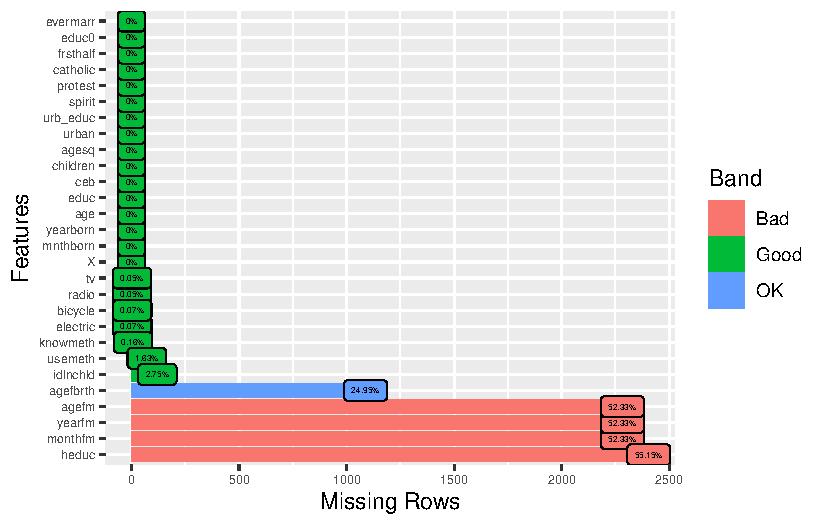
\includegraphics{Fertility_Rates_Education_Impact_Botswana_files/figure-pdf/unnamed-chunk-10-1.pdf}

}

\end{figure}

We can see how these missing values do not cause much of an issue since
these missing observations(parameters) convey less important information
than the other parameters. Hence we can ignore these values.

\#\#Removing missing values and parameters that are not required The aim
is to estimate the effect of education on women's fertility flexibly,
while controlling for possible linear and non-linear effects of
observable and unobservable confounding factors, and to analyse how the
effect of education changes when considering different expectiles of the
response variable distribution. We also include two variables regarding
the knowledge about and the use of birth control methods as well as
marital status.All three obviously influence the number of children.
Further, we include variables indicating wealth, e.g.~about the
availability of electricity, a television set or a bicycle.

Excluding variables that have no significant importance from our data.

\begin{Shaded}
\begin{Highlighting}[]
\NormalTok{Womendata }\OtherTok{\textless{}{-}} \FunctionTok{subset}\NormalTok{(Womendata, }\AttributeTok{select =} \SpecialCharTok{{-}}\FunctionTok{c}\NormalTok{(agefm,yearfm,monthfm,heduc))}
\end{Highlighting}
\end{Shaded}

\begin{Shaded}
\begin{Highlighting}[]
\NormalTok{Womendatacleaned }\OtherTok{\textless{}{-}}\NormalTok{Womendata[}\FunctionTok{complete.cases}\NormalTok{(Womendata), ]}
\FunctionTok{plot\_missing}\NormalTok{(}\AttributeTok{data =}\NormalTok{ Womendatacleaned, }\AttributeTok{geom\_label\_args =} \FunctionTok{list}\NormalTok{(}\AttributeTok{size =} \FloatTok{1.4}\NormalTok{), }\AttributeTok{theme\_config=}\FunctionTok{list}\NormalTok{(}\AttributeTok{axis.text=}\FunctionTok{element\_text}\NormalTok{(}\AttributeTok{size =} \DecValTok{6}\NormalTok{ )))}
\end{Highlighting}
\end{Shaded}

\begin{figure}[H]

{\centering 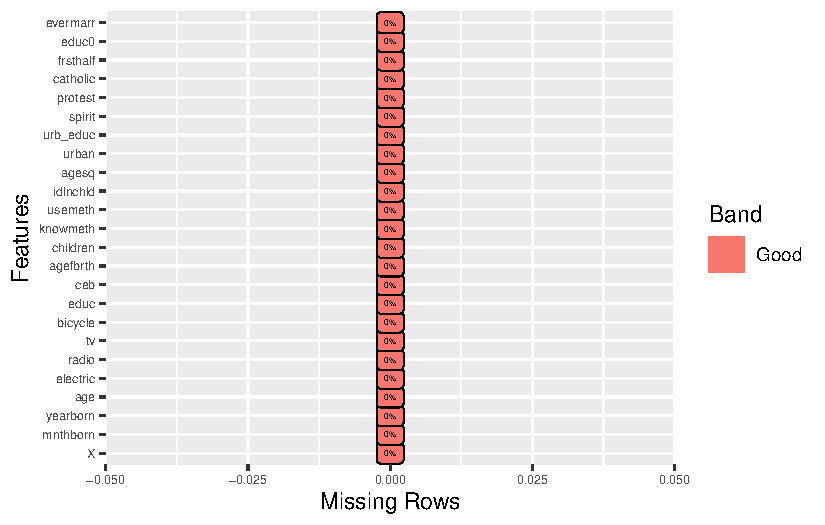
\includegraphics{Fertility_Rates_Education_Impact_Botswana_files/figure-pdf/unnamed-chunk-12-1.pdf}

}

\end{figure}

\hypertarget{detecting-outliers.}{%
\subsection{Detecting outliers.}\label{detecting-outliers.}}

\begin{Shaded}
\begin{Highlighting}[]
\NormalTok{Womendata }\SpecialCharTok{\%\textgreater{}\%}
  \FunctionTok{ggplot}\NormalTok{(}\FunctionTok{aes}\NormalTok{(educ)) }\SpecialCharTok{+}
  \FunctionTok{geom\_boxplot}\NormalTok{() }\SpecialCharTok{+}
  \FunctionTok{coord\_flip}\NormalTok{()}
\end{Highlighting}
\end{Shaded}

\begin{figure}[H]

{\centering 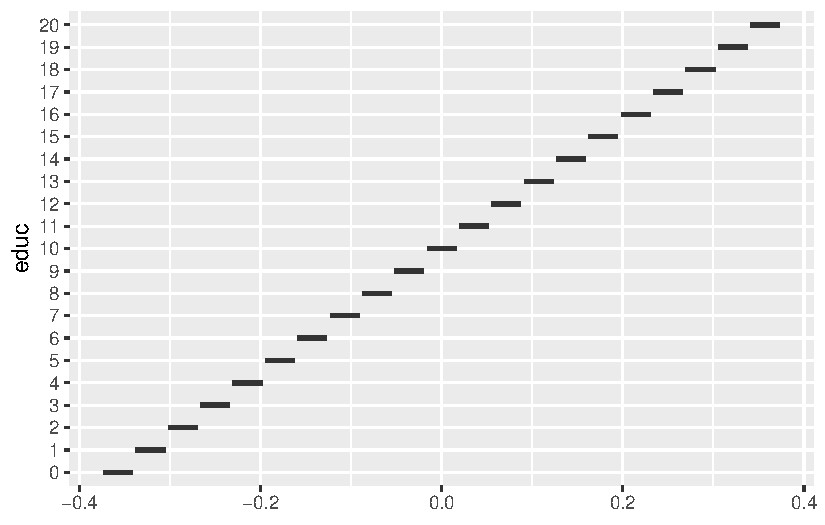
\includegraphics{Fertility_Rates_Education_Impact_Botswana_files/figure-pdf/unnamed-chunk-13-1.pdf}

}

\end{figure}

We can see that the variable educ i.e education has some outliers.
Mostly for having education of more than 15 years, but they cannot
potentially affect the data set.

\begin{Shaded}
\begin{Highlighting}[]
\NormalTok{Womendata }\SpecialCharTok{\%\textgreater{}\%}
  \FunctionTok{ggplot}\NormalTok{(}\FunctionTok{aes}\NormalTok{(age)) }\SpecialCharTok{+}
  \FunctionTok{geom\_boxplot}\NormalTok{() }\SpecialCharTok{+}
  \FunctionTok{coord\_flip}\NormalTok{()}
\end{Highlighting}
\end{Shaded}

\begin{figure}[H]

{\centering 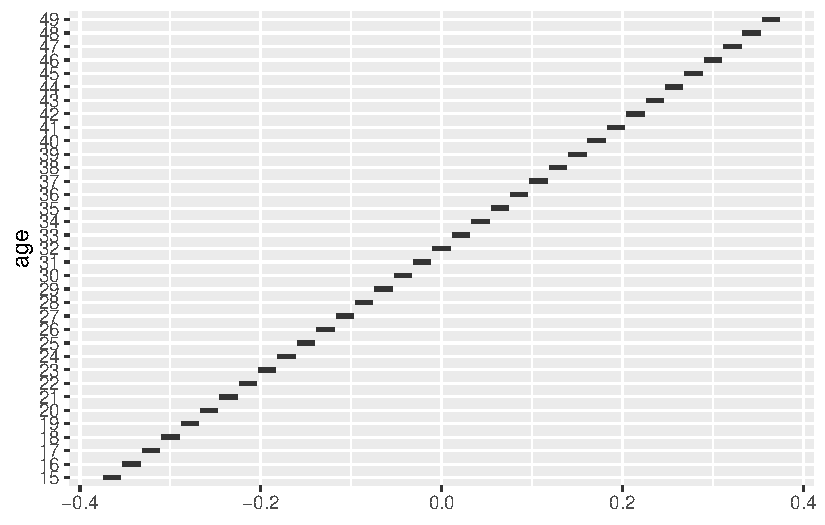
\includegraphics{Fertility_Rates_Education_Impact_Botswana_files/figure-pdf/unnamed-chunk-14-1.pdf}

}

\end{figure}

From above box plot, age variable has no outliers.

\begin{Shaded}
\begin{Highlighting}[]
\NormalTok{Womendata }\SpecialCharTok{\%\textgreater{}\%}
  \FunctionTok{ggplot}\NormalTok{(}\FunctionTok{aes}\NormalTok{(children)) }\SpecialCharTok{+}
  \FunctionTok{geom\_boxplot}\NormalTok{() }\SpecialCharTok{+}
  \FunctionTok{coord\_flip}\NormalTok{()}
\end{Highlighting}
\end{Shaded}

\begin{figure}[H]

{\centering 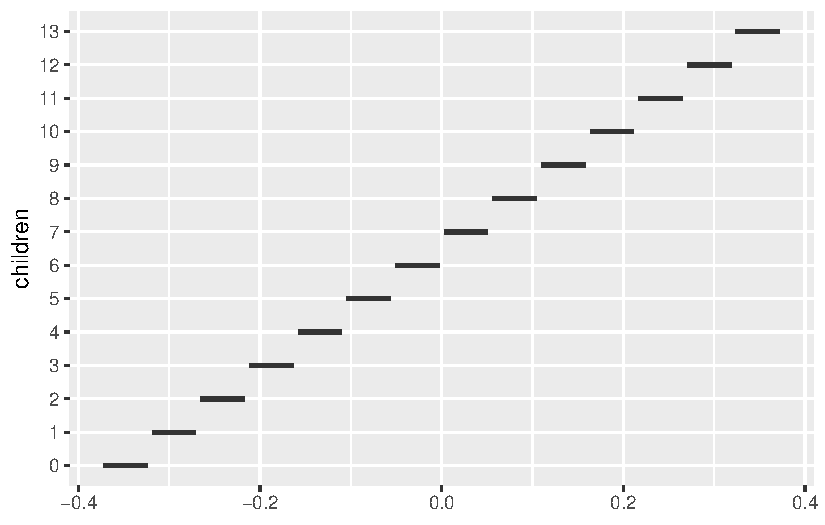
\includegraphics{Fertility_Rates_Education_Impact_Botswana_files/figure-pdf/unnamed-chunk-15-1.pdf}

}

\end{figure}

From the above plot we can see that the variable children does have
outliers but nothing to be concerned about.

\begin{Shaded}
\begin{Highlighting}[]
\NormalTok{Womendata }\SpecialCharTok{\%\textgreater{}\%}
  \FunctionTok{ggplot}\NormalTok{(}\FunctionTok{aes}\NormalTok{(urb\_educ)) }\SpecialCharTok{+}
  \FunctionTok{geom\_boxplot}\NormalTok{() }\SpecialCharTok{+}
  \FunctionTok{coord\_flip}\NormalTok{()}
\end{Highlighting}
\end{Shaded}

\begin{figure}[H]

{\centering 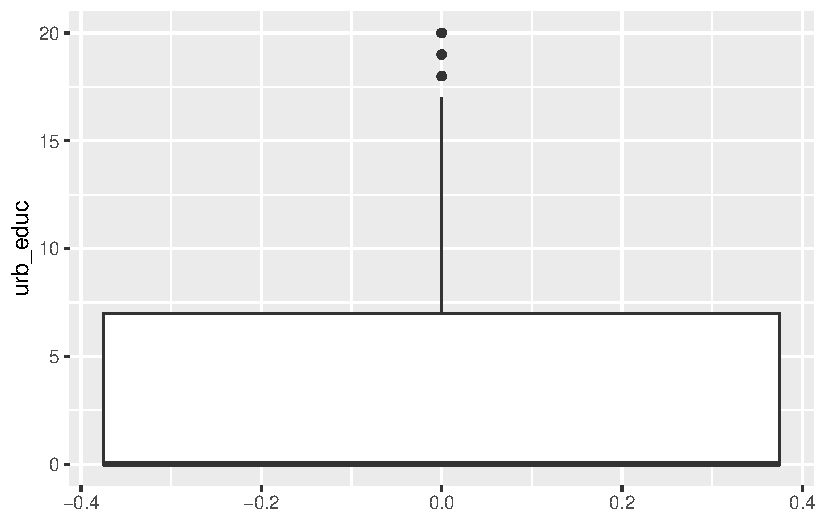
\includegraphics{Fertility_Rates_Education_Impact_Botswana_files/figure-pdf/unnamed-chunk-16-1.pdf}

}

\end{figure}

From the above plot we can see that the variable urban education does
have outliers but nothing to be concerned about.

\begin{Shaded}
\begin{Highlighting}[]
\NormalTok{Womendata }\SpecialCharTok{\%\textgreater{}\%}
  \FunctionTok{ggplot}\NormalTok{(}\FunctionTok{aes}\NormalTok{(yearborn)) }\SpecialCharTok{+}
  \FunctionTok{geom\_boxplot}\NormalTok{() }\SpecialCharTok{+}
  \FunctionTok{coord\_flip}\NormalTok{()}
\end{Highlighting}
\end{Shaded}

\begin{figure}[H]

{\centering 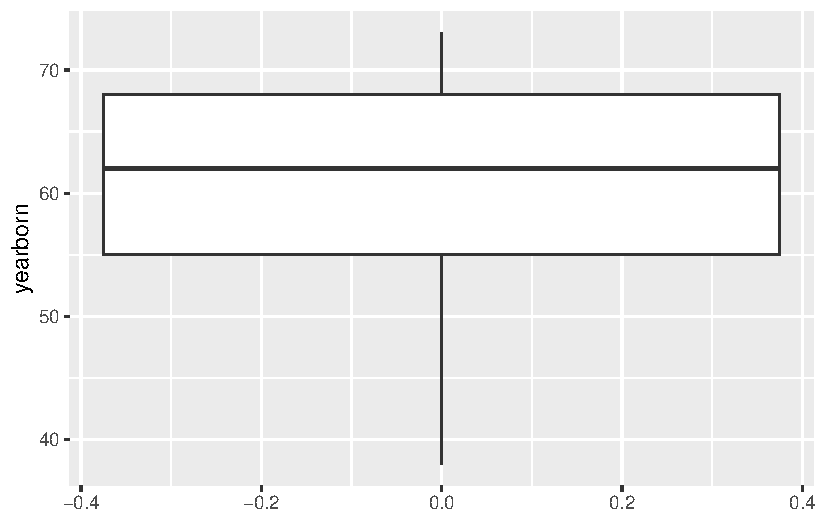
\includegraphics{Fertility_Rates_Education_Impact_Botswana_files/figure-pdf/unnamed-chunk-17-1.pdf}

}

\end{figure}

From the above box plot, yearborn variable has no outliers.

\begin{Shaded}
\begin{Highlighting}[]
\NormalTok{Womendata }\SpecialCharTok{\%\textgreater{}\%}
  \FunctionTok{ggplot}\NormalTok{(}\FunctionTok{aes}\NormalTok{(mnthborn)) }\SpecialCharTok{+}
  \FunctionTok{geom\_boxplot}\NormalTok{() }\SpecialCharTok{+}
  \FunctionTok{coord\_flip}\NormalTok{()}
\end{Highlighting}
\end{Shaded}

\begin{figure}[H]

{\centering 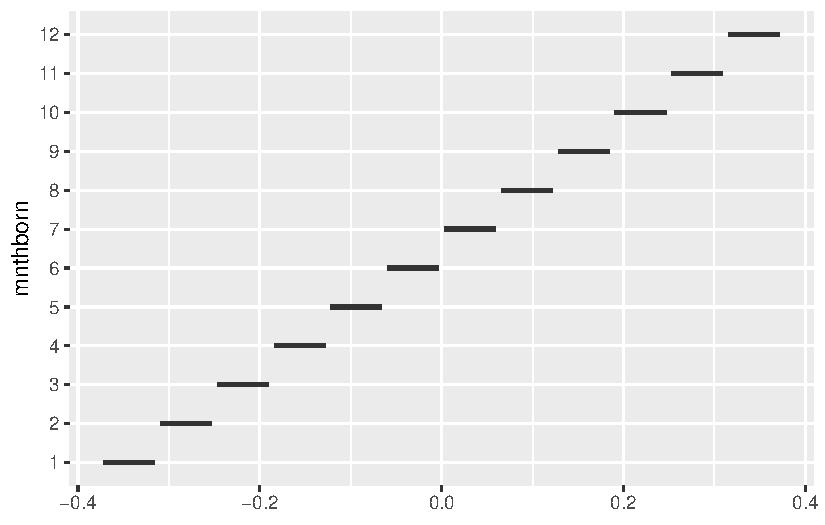
\includegraphics{Fertility_Rates_Education_Impact_Botswana_files/figure-pdf/unnamed-chunk-18-1.pdf}

}

\end{figure}

From the above box plot, mnthborn variable has no outliers.

\#Exploratory Data Analysis (EDA) EDA provided valuable insights into
the relationships between various variables and fertility rates.
Visualizations such as bar plots and box plots were used to understand
patterns and correlations.

\begin{Shaded}
\begin{Highlighting}[]
\FunctionTok{ggplot}\NormalTok{(Womendatacleaned,}\FunctionTok{aes}\NormalTok{(}\AttributeTok{x=}\FunctionTok{factor}\NormalTok{(children),}\AttributeTok{fill=}\FunctionTok{factor}\NormalTok{(tv)))}\SpecialCharTok{+}
  
\FunctionTok{geom\_bar}\NormalTok{()}\SpecialCharTok{+}\FunctionTok{theme}\NormalTok{(}\AttributeTok{axis.text.x =} \FunctionTok{element\_text}\NormalTok{(}\AttributeTok{face=}\StringTok{"bold"}\NormalTok{, }\AttributeTok{size=}\DecValTok{15}\NormalTok{),}\AttributeTok{axis.text.y =} \FunctionTok{element\_text}\NormalTok{(}\AttributeTok{face=}\StringTok{"bold"}\NormalTok{, }\AttributeTok{size=}\DecValTok{15}\NormalTok{))}\SpecialCharTok{+}
  
\FunctionTok{labs}\NormalTok{(}
    \AttributeTok{title =} \StringTok{"Number of Children based on if they own a Tv or not"}\NormalTok{,}
    \AttributeTok{x =} \StringTok{"Number of children"}\NormalTok{,}
    \AttributeTok{y =} \StringTok{"Count"}\NormalTok{,}\AttributeTok{size=}\DecValTok{15}\NormalTok{) }\SpecialCharTok{+}
   
\FunctionTok{scale\_fill\_manual}\NormalTok{(}
    \AttributeTok{name =} \StringTok{"Access to Telivision or not"}\NormalTok{,}
    \AttributeTok{breaks =} \FunctionTok{c}\NormalTok{(}\StringTok{"0"}\NormalTok{, }\StringTok{"1"}\NormalTok{),}
    \AttributeTok{labels =} \FunctionTok{c}\NormalTok{(}\StringTok{"No Telivision"}\NormalTok{, }\StringTok{"Owns/ has access to a telivision"}\NormalTok{),}
    \AttributeTok{values =} \FunctionTok{c}\NormalTok{(}\StringTok{"0"} \OtherTok{=} \StringTok{"orange"}\NormalTok{, }\StringTok{"1"}\OtherTok{=}\StringTok{"yellow"}\NormalTok{)}
\NormalTok{  )}
\end{Highlighting}
\end{Shaded}

\begin{figure}[H]

{\centering 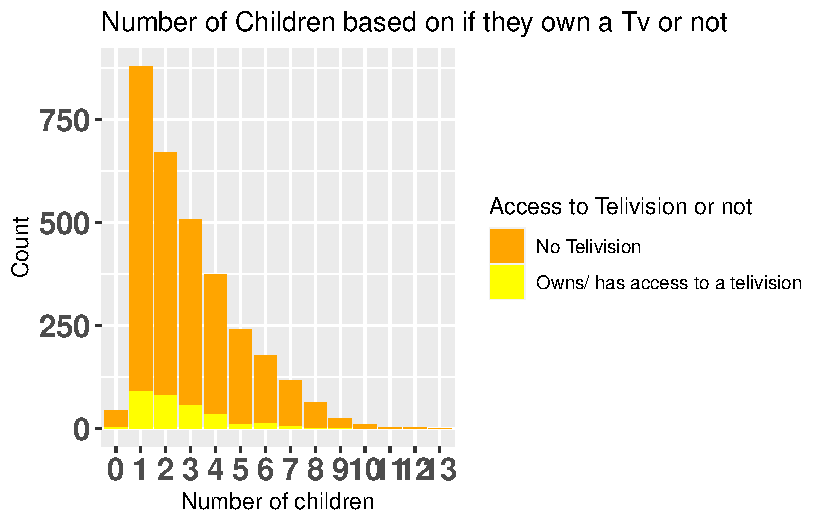
\includegraphics{Fertility_Rates_Education_Impact_Botswana_files/figure-pdf/unnamed-chunk-19-1.pdf}

}

\end{figure}

We can see that most mothers do not own a TV here.

\begin{Shaded}
\begin{Highlighting}[]
\FunctionTok{ggplot}\NormalTok{(Womendatacleaned,}\FunctionTok{aes}\NormalTok{(}\AttributeTok{x=}\FunctionTok{factor}\NormalTok{(children),}\AttributeTok{fill=}\FunctionTok{factor}\NormalTok{(radio)))}\SpecialCharTok{+}
  
\FunctionTok{geom\_bar}\NormalTok{()}\SpecialCharTok{+}\FunctionTok{theme}\NormalTok{(}\AttributeTok{axis.text.x =} \FunctionTok{element\_text}\NormalTok{(}\AttributeTok{face=}\StringTok{"bold"}\NormalTok{, }\AttributeTok{size=}\DecValTok{15}\NormalTok{),}\AttributeTok{axis.text.y =} \FunctionTok{element\_text}\NormalTok{(}\AttributeTok{face=}\StringTok{"bold"}\NormalTok{, }\AttributeTok{size=}\DecValTok{15}\NormalTok{))}\SpecialCharTok{+}
  
\FunctionTok{labs}\NormalTok{(}
    \AttributeTok{title =} \StringTok{"Number of Children based on if they own a radio or not"}\NormalTok{,}
    \AttributeTok{x =} \StringTok{"Number of children"}\NormalTok{,}
    \AttributeTok{y =} \StringTok{"Count"}\NormalTok{,}\AttributeTok{size=}\DecValTok{15}\NormalTok{) }\SpecialCharTok{+}
   
\FunctionTok{scale\_fill\_manual}\NormalTok{(}
    \AttributeTok{name =} \StringTok{"Access to Radio or not"}\NormalTok{,}
    \AttributeTok{breaks =} \FunctionTok{c}\NormalTok{(}\StringTok{"0"}\NormalTok{, }\StringTok{"1"}\NormalTok{),}
    \AttributeTok{labels =} \FunctionTok{c}\NormalTok{(}\StringTok{"No Radio"}\NormalTok{, }\StringTok{"Owns/ has access to a Radio"}\NormalTok{),}
    \AttributeTok{values =} \FunctionTok{c}\NormalTok{(}\StringTok{"0"} \OtherTok{=} \StringTok{"green"}\NormalTok{, }\StringTok{"1"}\OtherTok{=}\StringTok{"pink"}\NormalTok{)}
\NormalTok{  )}
\end{Highlighting}
\end{Shaded}

\begin{figure}[H]

{\centering 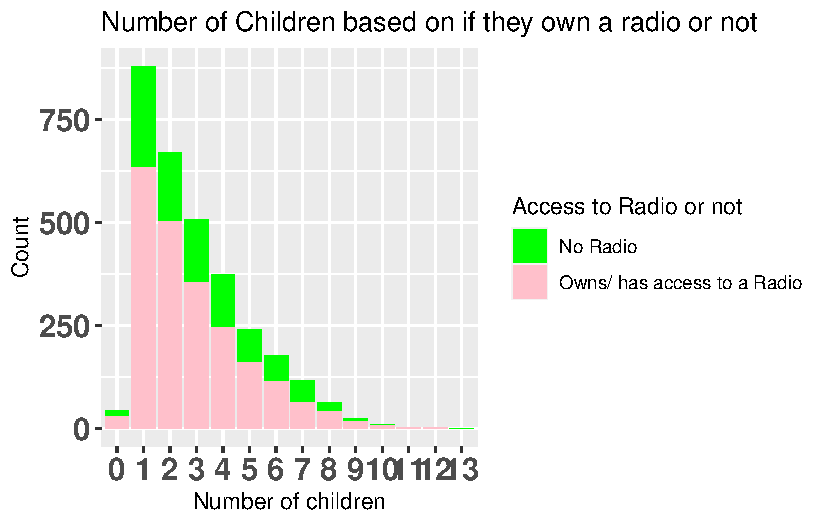
\includegraphics{Fertility_Rates_Education_Impact_Botswana_files/figure-pdf/unnamed-chunk-20-1.pdf}

}

\end{figure}

\begin{Shaded}
\begin{Highlighting}[]
\FunctionTok{ggplot}\NormalTok{(Womendatacleaned,}\FunctionTok{aes}\NormalTok{(}\AttributeTok{x=}\FunctionTok{factor}\NormalTok{(children),}\AttributeTok{fill=}\FunctionTok{factor}\NormalTok{(electric)))}\SpecialCharTok{+}
  
\FunctionTok{geom\_bar}\NormalTok{()}\SpecialCharTok{+}\FunctionTok{theme}\NormalTok{(}\AttributeTok{axis.text.x =} \FunctionTok{element\_text}\NormalTok{(}\AttributeTok{face=}\StringTok{"bold"}\NormalTok{, }\AttributeTok{size=}\DecValTok{15}\NormalTok{),}\AttributeTok{axis.text.y =} \FunctionTok{element\_text}\NormalTok{(}\AttributeTok{face=}\StringTok{"bold"}\NormalTok{, }\AttributeTok{size=}\DecValTok{15}\NormalTok{))}\SpecialCharTok{+}
  
\FunctionTok{labs}\NormalTok{(}
    \AttributeTok{title =} \StringTok{"Number of Children based on if they have electricity or not"}\NormalTok{,}
    \AttributeTok{x =} \StringTok{"Number of children"}\NormalTok{,}
    \AttributeTok{y =} \StringTok{"Count"}\NormalTok{,}\AttributeTok{size=}\DecValTok{15}\NormalTok{) }\SpecialCharTok{+}
   
\FunctionTok{scale\_fill\_manual}\NormalTok{(}
    \AttributeTok{name =} \StringTok{"Access to Electricity or not"}\NormalTok{,}
    \AttributeTok{breaks =} \FunctionTok{c}\NormalTok{(}\StringTok{"0"}\NormalTok{, }\StringTok{"1"}\NormalTok{),}
    \AttributeTok{labels =} \FunctionTok{c}\NormalTok{(}\StringTok{"No Electricity"}\NormalTok{, }\StringTok{"Has access to Electricity"}\NormalTok{),}
    \AttributeTok{values =} \FunctionTok{c}\NormalTok{(}\StringTok{"0"} \OtherTok{=} \StringTok{"pink"}\NormalTok{, }\StringTok{"1"}\OtherTok{=}\StringTok{"yellow"}\NormalTok{)}
\NormalTok{  )}
\end{Highlighting}
\end{Shaded}

\begin{figure}[H]

{\centering 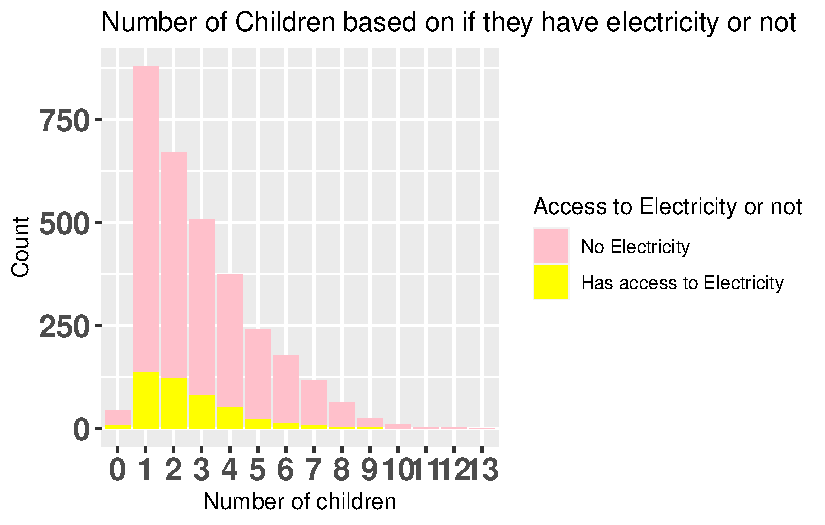
\includegraphics{Fertility_Rates_Education_Impact_Botswana_files/figure-pdf/unnamed-chunk-21-1.pdf}

}

\end{figure}

Here from our bar graph we can see that most mothers that have children
do not have electricity.

\begin{Shaded}
\begin{Highlighting}[]
\NormalTok{p }\OtherTok{\textless{}{-}}\NormalTok{ Womendata }\SpecialCharTok{\%\textgreater{}\%}
  \FunctionTok{ggplot}\NormalTok{() }\SpecialCharTok{+}
  \FunctionTok{geom\_bar}\NormalTok{(}\FunctionTok{aes}\NormalTok{(Womendata}\SpecialCharTok{$}\NormalTok{usemeth)) }\SpecialCharTok{+}
  \FunctionTok{ggtitle}\NormalTok{(}\StringTok{"Individuals that ever used birth control"}\NormalTok{) }\SpecialCharTok{+} \FunctionTok{labs}\NormalTok{(}\AttributeTok{title =} \StringTok{"Individuals that have ever used  birth control"}\NormalTok{, }
\AttributeTok{x =} \StringTok{"No. of individuals that have ever used birth control"}\NormalTok{,}\AttributeTok{y =} \StringTok{"Count"}\NormalTok{)}
  \FunctionTok{theme\_classic}\NormalTok{()}
\end{Highlighting}
\end{Shaded}

\begin{verbatim}
List of 97
 $ line                      :List of 6
  ..$ colour       : chr "black"
  ..$ linewidth    : num 0.5
  ..$ linetype     : num 1
  ..$ lineend      : chr "butt"
  ..$ arrow        : logi FALSE
  ..$ inherit.blank: logi TRUE
  ..- attr(*, "class")= chr [1:2] "element_line" "element"
 $ rect                      :List of 5
  ..$ fill         : chr "white"
  ..$ colour       : chr "black"
  ..$ linewidth    : num 0.5
  ..$ linetype     : num 1
  ..$ inherit.blank: logi TRUE
  ..- attr(*, "class")= chr [1:2] "element_rect" "element"
 $ text                      :List of 11
  ..$ family       : chr ""
  ..$ face         : chr "plain"
  ..$ colour       : chr "black"
  ..$ size         : num 11
  ..$ hjust        : num 0.5
  ..$ vjust        : num 0.5
  ..$ angle        : num 0
  ..$ lineheight   : num 0.9
  ..$ margin       : 'margin' num [1:4] 0points 0points 0points 0points
  .. ..- attr(*, "unit")= int 8
  ..$ debug        : logi FALSE
  ..$ inherit.blank: logi TRUE
  ..- attr(*, "class")= chr [1:2] "element_text" "element"
 $ title                     : NULL
 $ aspect.ratio              : NULL
 $ axis.title                : NULL
 $ axis.title.x              :List of 11
  ..$ family       : NULL
  ..$ face         : NULL
  ..$ colour       : NULL
  ..$ size         : NULL
  ..$ hjust        : NULL
  ..$ vjust        : num 1
  ..$ angle        : NULL
  ..$ lineheight   : NULL
  ..$ margin       : 'margin' num [1:4] 2.75points 0points 0points 0points
  .. ..- attr(*, "unit")= int 8
  ..$ debug        : NULL
  ..$ inherit.blank: logi TRUE
  ..- attr(*, "class")= chr [1:2] "element_text" "element"
 $ axis.title.x.top          :List of 11
  ..$ family       : NULL
  ..$ face         : NULL
  ..$ colour       : NULL
  ..$ size         : NULL
  ..$ hjust        : NULL
  ..$ vjust        : num 0
  ..$ angle        : NULL
  ..$ lineheight   : NULL
  ..$ margin       : 'margin' num [1:4] 0points 0points 2.75points 0points
  .. ..- attr(*, "unit")= int 8
  ..$ debug        : NULL
  ..$ inherit.blank: logi TRUE
  ..- attr(*, "class")= chr [1:2] "element_text" "element"
 $ axis.title.x.bottom       : NULL
 $ axis.title.y              :List of 11
  ..$ family       : NULL
  ..$ face         : NULL
  ..$ colour       : NULL
  ..$ size         : NULL
  ..$ hjust        : NULL
  ..$ vjust        : num 1
  ..$ angle        : num 90
  ..$ lineheight   : NULL
  ..$ margin       : 'margin' num [1:4] 0points 2.75points 0points 0points
  .. ..- attr(*, "unit")= int 8
  ..$ debug        : NULL
  ..$ inherit.blank: logi TRUE
  ..- attr(*, "class")= chr [1:2] "element_text" "element"
 $ axis.title.y.left         : NULL
 $ axis.title.y.right        :List of 11
  ..$ family       : NULL
  ..$ face         : NULL
  ..$ colour       : NULL
  ..$ size         : NULL
  ..$ hjust        : NULL
  ..$ vjust        : num 0
  ..$ angle        : num -90
  ..$ lineheight   : NULL
  ..$ margin       : 'margin' num [1:4] 0points 0points 0points 2.75points
  .. ..- attr(*, "unit")= int 8
  ..$ debug        : NULL
  ..$ inherit.blank: logi TRUE
  ..- attr(*, "class")= chr [1:2] "element_text" "element"
 $ axis.text                 :List of 11
  ..$ family       : NULL
  ..$ face         : NULL
  ..$ colour       : chr "grey30"
  ..$ size         : 'rel' num 0.8
  ..$ hjust        : NULL
  ..$ vjust        : NULL
  ..$ angle        : NULL
  ..$ lineheight   : NULL
  ..$ margin       : NULL
  ..$ debug        : NULL
  ..$ inherit.blank: logi TRUE
  ..- attr(*, "class")= chr [1:2] "element_text" "element"
 $ axis.text.x               :List of 11
  ..$ family       : NULL
  ..$ face         : NULL
  ..$ colour       : NULL
  ..$ size         : NULL
  ..$ hjust        : NULL
  ..$ vjust        : num 1
  ..$ angle        : NULL
  ..$ lineheight   : NULL
  ..$ margin       : 'margin' num [1:4] 2.2points 0points 0points 0points
  .. ..- attr(*, "unit")= int 8
  ..$ debug        : NULL
  ..$ inherit.blank: logi TRUE
  ..- attr(*, "class")= chr [1:2] "element_text" "element"
 $ axis.text.x.top           :List of 11
  ..$ family       : NULL
  ..$ face         : NULL
  ..$ colour       : NULL
  ..$ size         : NULL
  ..$ hjust        : NULL
  ..$ vjust        : num 0
  ..$ angle        : NULL
  ..$ lineheight   : NULL
  ..$ margin       : 'margin' num [1:4] 0points 0points 2.2points 0points
  .. ..- attr(*, "unit")= int 8
  ..$ debug        : NULL
  ..$ inherit.blank: logi TRUE
  ..- attr(*, "class")= chr [1:2] "element_text" "element"
 $ axis.text.x.bottom        : NULL
 $ axis.text.y               :List of 11
  ..$ family       : NULL
  ..$ face         : NULL
  ..$ colour       : NULL
  ..$ size         : NULL
  ..$ hjust        : num 1
  ..$ vjust        : NULL
  ..$ angle        : NULL
  ..$ lineheight   : NULL
  ..$ margin       : 'margin' num [1:4] 0points 2.2points 0points 0points
  .. ..- attr(*, "unit")= int 8
  ..$ debug        : NULL
  ..$ inherit.blank: logi TRUE
  ..- attr(*, "class")= chr [1:2] "element_text" "element"
 $ axis.text.y.left          : NULL
 $ axis.text.y.right         :List of 11
  ..$ family       : NULL
  ..$ face         : NULL
  ..$ colour       : NULL
  ..$ size         : NULL
  ..$ hjust        : num 0
  ..$ vjust        : NULL
  ..$ angle        : NULL
  ..$ lineheight   : NULL
  ..$ margin       : 'margin' num [1:4] 0points 0points 0points 2.2points
  .. ..- attr(*, "unit")= int 8
  ..$ debug        : NULL
  ..$ inherit.blank: logi TRUE
  ..- attr(*, "class")= chr [1:2] "element_text" "element"
 $ axis.ticks                :List of 6
  ..$ colour       : chr "grey20"
  ..$ linewidth    : NULL
  ..$ linetype     : NULL
  ..$ lineend      : NULL
  ..$ arrow        : logi FALSE
  ..$ inherit.blank: logi TRUE
  ..- attr(*, "class")= chr [1:2] "element_line" "element"
 $ axis.ticks.x              : NULL
 $ axis.ticks.x.top          : NULL
 $ axis.ticks.x.bottom       : NULL
 $ axis.ticks.y              : NULL
 $ axis.ticks.y.left         : NULL
 $ axis.ticks.y.right        : NULL
 $ axis.ticks.length         : 'simpleUnit' num 2.75points
  ..- attr(*, "unit")= int 8
 $ axis.ticks.length.x       : NULL
 $ axis.ticks.length.x.top   : NULL
 $ axis.ticks.length.x.bottom: NULL
 $ axis.ticks.length.y       : NULL
 $ axis.ticks.length.y.left  : NULL
 $ axis.ticks.length.y.right : NULL
 $ axis.line                 :List of 6
  ..$ colour       : chr "black"
  ..$ linewidth    : 'rel' num 1
  ..$ linetype     : NULL
  ..$ lineend      : NULL
  ..$ arrow        : logi FALSE
  ..$ inherit.blank: logi TRUE
  ..- attr(*, "class")= chr [1:2] "element_line" "element"
 $ axis.line.x               : NULL
 $ axis.line.x.top           : NULL
 $ axis.line.x.bottom        : NULL
 $ axis.line.y               : NULL
 $ axis.line.y.left          : NULL
 $ axis.line.y.right         : NULL
 $ legend.background         :List of 5
  ..$ fill         : NULL
  ..$ colour       : logi NA
  ..$ linewidth    : NULL
  ..$ linetype     : NULL
  ..$ inherit.blank: logi TRUE
  ..- attr(*, "class")= chr [1:2] "element_rect" "element"
 $ legend.margin             : 'margin' num [1:4] 5.5points 5.5points 5.5points 5.5points
  ..- attr(*, "unit")= int 8
 $ legend.spacing            : 'simpleUnit' num 11points
  ..- attr(*, "unit")= int 8
 $ legend.spacing.x          : NULL
 $ legend.spacing.y          : NULL
 $ legend.key                : list()
  ..- attr(*, "class")= chr [1:2] "element_blank" "element"
 $ legend.key.size           : 'simpleUnit' num 1.2lines
  ..- attr(*, "unit")= int 3
 $ legend.key.height         : NULL
 $ legend.key.width          : NULL
 $ legend.text               :List of 11
  ..$ family       : NULL
  ..$ face         : NULL
  ..$ colour       : NULL
  ..$ size         : 'rel' num 0.8
  ..$ hjust        : NULL
  ..$ vjust        : NULL
  ..$ angle        : NULL
  ..$ lineheight   : NULL
  ..$ margin       : NULL
  ..$ debug        : NULL
  ..$ inherit.blank: logi TRUE
  ..- attr(*, "class")= chr [1:2] "element_text" "element"
 $ legend.text.align         : NULL
 $ legend.title              :List of 11
  ..$ family       : NULL
  ..$ face         : NULL
  ..$ colour       : NULL
  ..$ size         : NULL
  ..$ hjust        : num 0
  ..$ vjust        : NULL
  ..$ angle        : NULL
  ..$ lineheight   : NULL
  ..$ margin       : NULL
  ..$ debug        : NULL
  ..$ inherit.blank: logi TRUE
  ..- attr(*, "class")= chr [1:2] "element_text" "element"
 $ legend.title.align        : NULL
 $ legend.position           : chr "right"
 $ legend.direction          : NULL
 $ legend.justification      : chr "center"
 $ legend.box                : NULL
 $ legend.box.just           : NULL
 $ legend.box.margin         : 'margin' num [1:4] 0cm 0cm 0cm 0cm
  ..- attr(*, "unit")= int 1
 $ legend.box.background     : list()
  ..- attr(*, "class")= chr [1:2] "element_blank" "element"
 $ legend.box.spacing        : 'simpleUnit' num 11points
  ..- attr(*, "unit")= int 8
 $ panel.background          :List of 5
  ..$ fill         : chr "white"
  ..$ colour       : logi NA
  ..$ linewidth    : NULL
  ..$ linetype     : NULL
  ..$ inherit.blank: logi TRUE
  ..- attr(*, "class")= chr [1:2] "element_rect" "element"
 $ panel.border              : list()
  ..- attr(*, "class")= chr [1:2] "element_blank" "element"
 $ panel.spacing             : 'simpleUnit' num 5.5points
  ..- attr(*, "unit")= int 8
 $ panel.spacing.x           : NULL
 $ panel.spacing.y           : NULL
 $ panel.grid                :List of 6
  ..$ colour       : chr "grey92"
  ..$ linewidth    : NULL
  ..$ linetype     : NULL
  ..$ lineend      : NULL
  ..$ arrow        : logi FALSE
  ..$ inherit.blank: logi TRUE
  ..- attr(*, "class")= chr [1:2] "element_line" "element"
 $ panel.grid.major          : list()
  ..- attr(*, "class")= chr [1:2] "element_blank" "element"
 $ panel.grid.minor          : list()
  ..- attr(*, "class")= chr [1:2] "element_blank" "element"
 $ panel.grid.major.x        : NULL
 $ panel.grid.major.y        : NULL
 $ panel.grid.minor.x        : NULL
 $ panel.grid.minor.y        : NULL
 $ panel.ontop               : logi FALSE
 $ plot.background           :List of 5
  ..$ fill         : NULL
  ..$ colour       : chr "white"
  ..$ linewidth    : NULL
  ..$ linetype     : NULL
  ..$ inherit.blank: logi TRUE
  ..- attr(*, "class")= chr [1:2] "element_rect" "element"
 $ plot.title                :List of 11
  ..$ family       : NULL
  ..$ face         : NULL
  ..$ colour       : NULL
  ..$ size         : 'rel' num 1.2
  ..$ hjust        : num 0
  ..$ vjust        : num 1
  ..$ angle        : NULL
  ..$ lineheight   : NULL
  ..$ margin       : 'margin' num [1:4] 0points 0points 5.5points 0points
  .. ..- attr(*, "unit")= int 8
  ..$ debug        : NULL
  ..$ inherit.blank: logi TRUE
  ..- attr(*, "class")= chr [1:2] "element_text" "element"
 $ plot.title.position       : chr "panel"
 $ plot.subtitle             :List of 11
  ..$ family       : NULL
  ..$ face         : NULL
  ..$ colour       : NULL
  ..$ size         : NULL
  ..$ hjust        : num 0
  ..$ vjust        : num 1
  ..$ angle        : NULL
  ..$ lineheight   : NULL
  ..$ margin       : 'margin' num [1:4] 0points 0points 5.5points 0points
  .. ..- attr(*, "unit")= int 8
  ..$ debug        : NULL
  ..$ inherit.blank: logi TRUE
  ..- attr(*, "class")= chr [1:2] "element_text" "element"
 $ plot.caption              :List of 11
  ..$ family       : NULL
  ..$ face         : NULL
  ..$ colour       : NULL
  ..$ size         : 'rel' num 0.8
  ..$ hjust        : num 1
  ..$ vjust        : num 1
  ..$ angle        : NULL
  ..$ lineheight   : NULL
  ..$ margin       : 'margin' num [1:4] 5.5points 0points 0points 0points
  .. ..- attr(*, "unit")= int 8
  ..$ debug        : NULL
  ..$ inherit.blank: logi TRUE
  ..- attr(*, "class")= chr [1:2] "element_text" "element"
 $ plot.caption.position     : chr "panel"
 $ plot.tag                  :List of 11
  ..$ family       : NULL
  ..$ face         : NULL
  ..$ colour       : NULL
  ..$ size         : 'rel' num 1.2
  ..$ hjust        : num 0.5
  ..$ vjust        : num 0.5
  ..$ angle        : NULL
  ..$ lineheight   : NULL
  ..$ margin       : NULL
  ..$ debug        : NULL
  ..$ inherit.blank: logi TRUE
  ..- attr(*, "class")= chr [1:2] "element_text" "element"
 $ plot.tag.position         : chr "topleft"
 $ plot.margin               : 'margin' num [1:4] 5.5points 5.5points 5.5points 5.5points
  ..- attr(*, "unit")= int 8
 $ strip.background          :List of 5
  ..$ fill         : chr "white"
  ..$ colour       : chr "black"
  ..$ linewidth    : 'rel' num 2
  ..$ linetype     : NULL
  ..$ inherit.blank: logi TRUE
  ..- attr(*, "class")= chr [1:2] "element_rect" "element"
 $ strip.background.x        : NULL
 $ strip.background.y        : NULL
 $ strip.clip                : chr "inherit"
 $ strip.placement           : chr "inside"
 $ strip.text                :List of 11
  ..$ family       : NULL
  ..$ face         : NULL
  ..$ colour       : chr "grey10"
  ..$ size         : 'rel' num 0.8
  ..$ hjust        : NULL
  ..$ vjust        : NULL
  ..$ angle        : NULL
  ..$ lineheight   : NULL
  ..$ margin       : 'margin' num [1:4] 4.4points 4.4points 4.4points 4.4points
  .. ..- attr(*, "unit")= int 8
  ..$ debug        : NULL
  ..$ inherit.blank: logi TRUE
  ..- attr(*, "class")= chr [1:2] "element_text" "element"
 $ strip.text.x              : NULL
 $ strip.text.x.bottom       : NULL
 $ strip.text.x.top          : NULL
 $ strip.text.y              :List of 11
  ..$ family       : NULL
  ..$ face         : NULL
  ..$ colour       : NULL
  ..$ size         : NULL
  ..$ hjust        : NULL
  ..$ vjust        : NULL
  ..$ angle        : num -90
  ..$ lineheight   : NULL
  ..$ margin       : NULL
  ..$ debug        : NULL
  ..$ inherit.blank: logi TRUE
  ..- attr(*, "class")= chr [1:2] "element_text" "element"
 $ strip.text.y.left         :List of 11
  ..$ family       : NULL
  ..$ face         : NULL
  ..$ colour       : NULL
  ..$ size         : NULL
  ..$ hjust        : NULL
  ..$ vjust        : NULL
  ..$ angle        : num 90
  ..$ lineheight   : NULL
  ..$ margin       : NULL
  ..$ debug        : NULL
  ..$ inherit.blank: logi TRUE
  ..- attr(*, "class")= chr [1:2] "element_text" "element"
 $ strip.text.y.right        : NULL
 $ strip.switch.pad.grid     : 'simpleUnit' num 2.75points
  ..- attr(*, "unit")= int 8
 $ strip.switch.pad.wrap     : 'simpleUnit' num 2.75points
  ..- attr(*, "unit")= int 8
 - attr(*, "class")= chr [1:2] "theme" "gg"
 - attr(*, "complete")= logi TRUE
 - attr(*, "validate")= logi TRUE
\end{verbatim}

\begin{Shaded}
\begin{Highlighting}[]
\NormalTok{p}
\end{Highlighting}
\end{Shaded}

\begin{verbatim}
Warning: Use of `Womendata$usemeth` is discouraged.
i Use `usemeth` instead.
\end{verbatim}

\begin{verbatim}
Warning: Removed 71 rows containing non-finite values (`stat_count()`).
\end{verbatim}

\begin{figure}[H]

{\centering 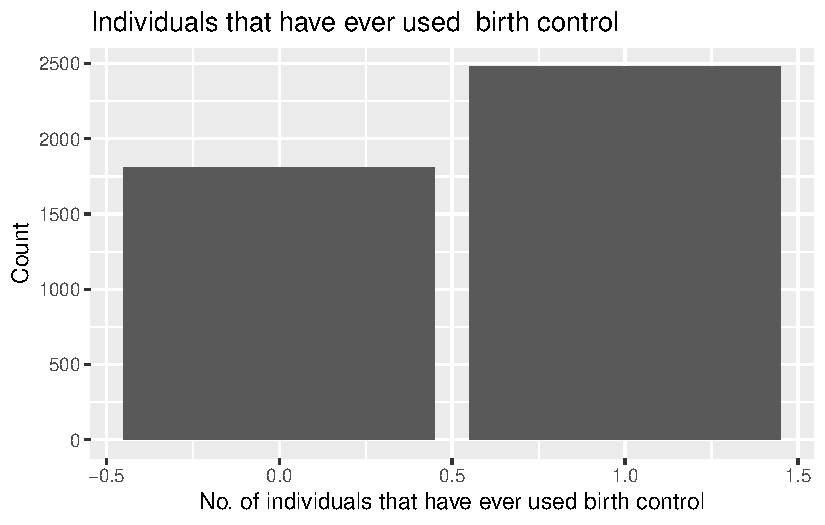
\includegraphics{Fertility_Rates_Education_Impact_Botswana_files/figure-pdf/unnamed-chunk-22-1.pdf}

}

\end{figure}

Majority of women have used birth control atleast once in their life.

\begin{Shaded}
\begin{Highlighting}[]
\NormalTok{k }\OtherTok{\textless{}{-}}\NormalTok{ Womendata }\SpecialCharTok{\%\textgreater{}\%}
  \FunctionTok{ggplot}\NormalTok{() }\SpecialCharTok{+}
  \FunctionTok{geom\_bar}\NormalTok{(}\FunctionTok{aes}\NormalTok{(Womendata}\SpecialCharTok{$}\NormalTok{knowmeth)) }\SpecialCharTok{+}
  \FunctionTok{ggtitle}\NormalTok{(}\StringTok{"Individuals that know about birth control"}\NormalTok{) }\SpecialCharTok{+} \FunctionTok{labs}\NormalTok{(}\AttributeTok{title =} \StringTok{"Individual knows about birth control"}\NormalTok{, }
\AttributeTok{x =} \StringTok{"No. of individuals that know about birth control"}\NormalTok{,}\AttributeTok{y =} \StringTok{"Count"}\NormalTok{)}
  \FunctionTok{theme\_classic}\NormalTok{()}
\end{Highlighting}
\end{Shaded}

\begin{verbatim}
List of 97
 $ line                      :List of 6
  ..$ colour       : chr "black"
  ..$ linewidth    : num 0.5
  ..$ linetype     : num 1
  ..$ lineend      : chr "butt"
  ..$ arrow        : logi FALSE
  ..$ inherit.blank: logi TRUE
  ..- attr(*, "class")= chr [1:2] "element_line" "element"
 $ rect                      :List of 5
  ..$ fill         : chr "white"
  ..$ colour       : chr "black"
  ..$ linewidth    : num 0.5
  ..$ linetype     : num 1
  ..$ inherit.blank: logi TRUE
  ..- attr(*, "class")= chr [1:2] "element_rect" "element"
 $ text                      :List of 11
  ..$ family       : chr ""
  ..$ face         : chr "plain"
  ..$ colour       : chr "black"
  ..$ size         : num 11
  ..$ hjust        : num 0.5
  ..$ vjust        : num 0.5
  ..$ angle        : num 0
  ..$ lineheight   : num 0.9
  ..$ margin       : 'margin' num [1:4] 0points 0points 0points 0points
  .. ..- attr(*, "unit")= int 8
  ..$ debug        : logi FALSE
  ..$ inherit.blank: logi TRUE
  ..- attr(*, "class")= chr [1:2] "element_text" "element"
 $ title                     : NULL
 $ aspect.ratio              : NULL
 $ axis.title                : NULL
 $ axis.title.x              :List of 11
  ..$ family       : NULL
  ..$ face         : NULL
  ..$ colour       : NULL
  ..$ size         : NULL
  ..$ hjust        : NULL
  ..$ vjust        : num 1
  ..$ angle        : NULL
  ..$ lineheight   : NULL
  ..$ margin       : 'margin' num [1:4] 2.75points 0points 0points 0points
  .. ..- attr(*, "unit")= int 8
  ..$ debug        : NULL
  ..$ inherit.blank: logi TRUE
  ..- attr(*, "class")= chr [1:2] "element_text" "element"
 $ axis.title.x.top          :List of 11
  ..$ family       : NULL
  ..$ face         : NULL
  ..$ colour       : NULL
  ..$ size         : NULL
  ..$ hjust        : NULL
  ..$ vjust        : num 0
  ..$ angle        : NULL
  ..$ lineheight   : NULL
  ..$ margin       : 'margin' num [1:4] 0points 0points 2.75points 0points
  .. ..- attr(*, "unit")= int 8
  ..$ debug        : NULL
  ..$ inherit.blank: logi TRUE
  ..- attr(*, "class")= chr [1:2] "element_text" "element"
 $ axis.title.x.bottom       : NULL
 $ axis.title.y              :List of 11
  ..$ family       : NULL
  ..$ face         : NULL
  ..$ colour       : NULL
  ..$ size         : NULL
  ..$ hjust        : NULL
  ..$ vjust        : num 1
  ..$ angle        : num 90
  ..$ lineheight   : NULL
  ..$ margin       : 'margin' num [1:4] 0points 2.75points 0points 0points
  .. ..- attr(*, "unit")= int 8
  ..$ debug        : NULL
  ..$ inherit.blank: logi TRUE
  ..- attr(*, "class")= chr [1:2] "element_text" "element"
 $ axis.title.y.left         : NULL
 $ axis.title.y.right        :List of 11
  ..$ family       : NULL
  ..$ face         : NULL
  ..$ colour       : NULL
  ..$ size         : NULL
  ..$ hjust        : NULL
  ..$ vjust        : num 0
  ..$ angle        : num -90
  ..$ lineheight   : NULL
  ..$ margin       : 'margin' num [1:4] 0points 0points 0points 2.75points
  .. ..- attr(*, "unit")= int 8
  ..$ debug        : NULL
  ..$ inherit.blank: logi TRUE
  ..- attr(*, "class")= chr [1:2] "element_text" "element"
 $ axis.text                 :List of 11
  ..$ family       : NULL
  ..$ face         : NULL
  ..$ colour       : chr "grey30"
  ..$ size         : 'rel' num 0.8
  ..$ hjust        : NULL
  ..$ vjust        : NULL
  ..$ angle        : NULL
  ..$ lineheight   : NULL
  ..$ margin       : NULL
  ..$ debug        : NULL
  ..$ inherit.blank: logi TRUE
  ..- attr(*, "class")= chr [1:2] "element_text" "element"
 $ axis.text.x               :List of 11
  ..$ family       : NULL
  ..$ face         : NULL
  ..$ colour       : NULL
  ..$ size         : NULL
  ..$ hjust        : NULL
  ..$ vjust        : num 1
  ..$ angle        : NULL
  ..$ lineheight   : NULL
  ..$ margin       : 'margin' num [1:4] 2.2points 0points 0points 0points
  .. ..- attr(*, "unit")= int 8
  ..$ debug        : NULL
  ..$ inherit.blank: logi TRUE
  ..- attr(*, "class")= chr [1:2] "element_text" "element"
 $ axis.text.x.top           :List of 11
  ..$ family       : NULL
  ..$ face         : NULL
  ..$ colour       : NULL
  ..$ size         : NULL
  ..$ hjust        : NULL
  ..$ vjust        : num 0
  ..$ angle        : NULL
  ..$ lineheight   : NULL
  ..$ margin       : 'margin' num [1:4] 0points 0points 2.2points 0points
  .. ..- attr(*, "unit")= int 8
  ..$ debug        : NULL
  ..$ inherit.blank: logi TRUE
  ..- attr(*, "class")= chr [1:2] "element_text" "element"
 $ axis.text.x.bottom        : NULL
 $ axis.text.y               :List of 11
  ..$ family       : NULL
  ..$ face         : NULL
  ..$ colour       : NULL
  ..$ size         : NULL
  ..$ hjust        : num 1
  ..$ vjust        : NULL
  ..$ angle        : NULL
  ..$ lineheight   : NULL
  ..$ margin       : 'margin' num [1:4] 0points 2.2points 0points 0points
  .. ..- attr(*, "unit")= int 8
  ..$ debug        : NULL
  ..$ inherit.blank: logi TRUE
  ..- attr(*, "class")= chr [1:2] "element_text" "element"
 $ axis.text.y.left          : NULL
 $ axis.text.y.right         :List of 11
  ..$ family       : NULL
  ..$ face         : NULL
  ..$ colour       : NULL
  ..$ size         : NULL
  ..$ hjust        : num 0
  ..$ vjust        : NULL
  ..$ angle        : NULL
  ..$ lineheight   : NULL
  ..$ margin       : 'margin' num [1:4] 0points 0points 0points 2.2points
  .. ..- attr(*, "unit")= int 8
  ..$ debug        : NULL
  ..$ inherit.blank: logi TRUE
  ..- attr(*, "class")= chr [1:2] "element_text" "element"
 $ axis.ticks                :List of 6
  ..$ colour       : chr "grey20"
  ..$ linewidth    : NULL
  ..$ linetype     : NULL
  ..$ lineend      : NULL
  ..$ arrow        : logi FALSE
  ..$ inherit.blank: logi TRUE
  ..- attr(*, "class")= chr [1:2] "element_line" "element"
 $ axis.ticks.x              : NULL
 $ axis.ticks.x.top          : NULL
 $ axis.ticks.x.bottom       : NULL
 $ axis.ticks.y              : NULL
 $ axis.ticks.y.left         : NULL
 $ axis.ticks.y.right        : NULL
 $ axis.ticks.length         : 'simpleUnit' num 2.75points
  ..- attr(*, "unit")= int 8
 $ axis.ticks.length.x       : NULL
 $ axis.ticks.length.x.top   : NULL
 $ axis.ticks.length.x.bottom: NULL
 $ axis.ticks.length.y       : NULL
 $ axis.ticks.length.y.left  : NULL
 $ axis.ticks.length.y.right : NULL
 $ axis.line                 :List of 6
  ..$ colour       : chr "black"
  ..$ linewidth    : 'rel' num 1
  ..$ linetype     : NULL
  ..$ lineend      : NULL
  ..$ arrow        : logi FALSE
  ..$ inherit.blank: logi TRUE
  ..- attr(*, "class")= chr [1:2] "element_line" "element"
 $ axis.line.x               : NULL
 $ axis.line.x.top           : NULL
 $ axis.line.x.bottom        : NULL
 $ axis.line.y               : NULL
 $ axis.line.y.left          : NULL
 $ axis.line.y.right         : NULL
 $ legend.background         :List of 5
  ..$ fill         : NULL
  ..$ colour       : logi NA
  ..$ linewidth    : NULL
  ..$ linetype     : NULL
  ..$ inherit.blank: logi TRUE
  ..- attr(*, "class")= chr [1:2] "element_rect" "element"
 $ legend.margin             : 'margin' num [1:4] 5.5points 5.5points 5.5points 5.5points
  ..- attr(*, "unit")= int 8
 $ legend.spacing            : 'simpleUnit' num 11points
  ..- attr(*, "unit")= int 8
 $ legend.spacing.x          : NULL
 $ legend.spacing.y          : NULL
 $ legend.key                : list()
  ..- attr(*, "class")= chr [1:2] "element_blank" "element"
 $ legend.key.size           : 'simpleUnit' num 1.2lines
  ..- attr(*, "unit")= int 3
 $ legend.key.height         : NULL
 $ legend.key.width          : NULL
 $ legend.text               :List of 11
  ..$ family       : NULL
  ..$ face         : NULL
  ..$ colour       : NULL
  ..$ size         : 'rel' num 0.8
  ..$ hjust        : NULL
  ..$ vjust        : NULL
  ..$ angle        : NULL
  ..$ lineheight   : NULL
  ..$ margin       : NULL
  ..$ debug        : NULL
  ..$ inherit.blank: logi TRUE
  ..- attr(*, "class")= chr [1:2] "element_text" "element"
 $ legend.text.align         : NULL
 $ legend.title              :List of 11
  ..$ family       : NULL
  ..$ face         : NULL
  ..$ colour       : NULL
  ..$ size         : NULL
  ..$ hjust        : num 0
  ..$ vjust        : NULL
  ..$ angle        : NULL
  ..$ lineheight   : NULL
  ..$ margin       : NULL
  ..$ debug        : NULL
  ..$ inherit.blank: logi TRUE
  ..- attr(*, "class")= chr [1:2] "element_text" "element"
 $ legend.title.align        : NULL
 $ legend.position           : chr "right"
 $ legend.direction          : NULL
 $ legend.justification      : chr "center"
 $ legend.box                : NULL
 $ legend.box.just           : NULL
 $ legend.box.margin         : 'margin' num [1:4] 0cm 0cm 0cm 0cm
  ..- attr(*, "unit")= int 1
 $ legend.box.background     : list()
  ..- attr(*, "class")= chr [1:2] "element_blank" "element"
 $ legend.box.spacing        : 'simpleUnit' num 11points
  ..- attr(*, "unit")= int 8
 $ panel.background          :List of 5
  ..$ fill         : chr "white"
  ..$ colour       : logi NA
  ..$ linewidth    : NULL
  ..$ linetype     : NULL
  ..$ inherit.blank: logi TRUE
  ..- attr(*, "class")= chr [1:2] "element_rect" "element"
 $ panel.border              : list()
  ..- attr(*, "class")= chr [1:2] "element_blank" "element"
 $ panel.spacing             : 'simpleUnit' num 5.5points
  ..- attr(*, "unit")= int 8
 $ panel.spacing.x           : NULL
 $ panel.spacing.y           : NULL
 $ panel.grid                :List of 6
  ..$ colour       : chr "grey92"
  ..$ linewidth    : NULL
  ..$ linetype     : NULL
  ..$ lineend      : NULL
  ..$ arrow        : logi FALSE
  ..$ inherit.blank: logi TRUE
  ..- attr(*, "class")= chr [1:2] "element_line" "element"
 $ panel.grid.major          : list()
  ..- attr(*, "class")= chr [1:2] "element_blank" "element"
 $ panel.grid.minor          : list()
  ..- attr(*, "class")= chr [1:2] "element_blank" "element"
 $ panel.grid.major.x        : NULL
 $ panel.grid.major.y        : NULL
 $ panel.grid.minor.x        : NULL
 $ panel.grid.minor.y        : NULL
 $ panel.ontop               : logi FALSE
 $ plot.background           :List of 5
  ..$ fill         : NULL
  ..$ colour       : chr "white"
  ..$ linewidth    : NULL
  ..$ linetype     : NULL
  ..$ inherit.blank: logi TRUE
  ..- attr(*, "class")= chr [1:2] "element_rect" "element"
 $ plot.title                :List of 11
  ..$ family       : NULL
  ..$ face         : NULL
  ..$ colour       : NULL
  ..$ size         : 'rel' num 1.2
  ..$ hjust        : num 0
  ..$ vjust        : num 1
  ..$ angle        : NULL
  ..$ lineheight   : NULL
  ..$ margin       : 'margin' num [1:4] 0points 0points 5.5points 0points
  .. ..- attr(*, "unit")= int 8
  ..$ debug        : NULL
  ..$ inherit.blank: logi TRUE
  ..- attr(*, "class")= chr [1:2] "element_text" "element"
 $ plot.title.position       : chr "panel"
 $ plot.subtitle             :List of 11
  ..$ family       : NULL
  ..$ face         : NULL
  ..$ colour       : NULL
  ..$ size         : NULL
  ..$ hjust        : num 0
  ..$ vjust        : num 1
  ..$ angle        : NULL
  ..$ lineheight   : NULL
  ..$ margin       : 'margin' num [1:4] 0points 0points 5.5points 0points
  .. ..- attr(*, "unit")= int 8
  ..$ debug        : NULL
  ..$ inherit.blank: logi TRUE
  ..- attr(*, "class")= chr [1:2] "element_text" "element"
 $ plot.caption              :List of 11
  ..$ family       : NULL
  ..$ face         : NULL
  ..$ colour       : NULL
  ..$ size         : 'rel' num 0.8
  ..$ hjust        : num 1
  ..$ vjust        : num 1
  ..$ angle        : NULL
  ..$ lineheight   : NULL
  ..$ margin       : 'margin' num [1:4] 5.5points 0points 0points 0points
  .. ..- attr(*, "unit")= int 8
  ..$ debug        : NULL
  ..$ inherit.blank: logi TRUE
  ..- attr(*, "class")= chr [1:2] "element_text" "element"
 $ plot.caption.position     : chr "panel"
 $ plot.tag                  :List of 11
  ..$ family       : NULL
  ..$ face         : NULL
  ..$ colour       : NULL
  ..$ size         : 'rel' num 1.2
  ..$ hjust        : num 0.5
  ..$ vjust        : num 0.5
  ..$ angle        : NULL
  ..$ lineheight   : NULL
  ..$ margin       : NULL
  ..$ debug        : NULL
  ..$ inherit.blank: logi TRUE
  ..- attr(*, "class")= chr [1:2] "element_text" "element"
 $ plot.tag.position         : chr "topleft"
 $ plot.margin               : 'margin' num [1:4] 5.5points 5.5points 5.5points 5.5points
  ..- attr(*, "unit")= int 8
 $ strip.background          :List of 5
  ..$ fill         : chr "white"
  ..$ colour       : chr "black"
  ..$ linewidth    : 'rel' num 2
  ..$ linetype     : NULL
  ..$ inherit.blank: logi TRUE
  ..- attr(*, "class")= chr [1:2] "element_rect" "element"
 $ strip.background.x        : NULL
 $ strip.background.y        : NULL
 $ strip.clip                : chr "inherit"
 $ strip.placement           : chr "inside"
 $ strip.text                :List of 11
  ..$ family       : NULL
  ..$ face         : NULL
  ..$ colour       : chr "grey10"
  ..$ size         : 'rel' num 0.8
  ..$ hjust        : NULL
  ..$ vjust        : NULL
  ..$ angle        : NULL
  ..$ lineheight   : NULL
  ..$ margin       : 'margin' num [1:4] 4.4points 4.4points 4.4points 4.4points
  .. ..- attr(*, "unit")= int 8
  ..$ debug        : NULL
  ..$ inherit.blank: logi TRUE
  ..- attr(*, "class")= chr [1:2] "element_text" "element"
 $ strip.text.x              : NULL
 $ strip.text.x.bottom       : NULL
 $ strip.text.x.top          : NULL
 $ strip.text.y              :List of 11
  ..$ family       : NULL
  ..$ face         : NULL
  ..$ colour       : NULL
  ..$ size         : NULL
  ..$ hjust        : NULL
  ..$ vjust        : NULL
  ..$ angle        : num -90
  ..$ lineheight   : NULL
  ..$ margin       : NULL
  ..$ debug        : NULL
  ..$ inherit.blank: logi TRUE
  ..- attr(*, "class")= chr [1:2] "element_text" "element"
 $ strip.text.y.left         :List of 11
  ..$ family       : NULL
  ..$ face         : NULL
  ..$ colour       : NULL
  ..$ size         : NULL
  ..$ hjust        : NULL
  ..$ vjust        : NULL
  ..$ angle        : num 90
  ..$ lineheight   : NULL
  ..$ margin       : NULL
  ..$ debug        : NULL
  ..$ inherit.blank: logi TRUE
  ..- attr(*, "class")= chr [1:2] "element_text" "element"
 $ strip.text.y.right        : NULL
 $ strip.switch.pad.grid     : 'simpleUnit' num 2.75points
  ..- attr(*, "unit")= int 8
 $ strip.switch.pad.wrap     : 'simpleUnit' num 2.75points
  ..- attr(*, "unit")= int 8
 - attr(*, "class")= chr [1:2] "theme" "gg"
 - attr(*, "complete")= logi TRUE
 - attr(*, "validate")= logi TRUE
\end{verbatim}

\begin{Shaded}
\begin{Highlighting}[]
\NormalTok{k}
\end{Highlighting}
\end{Shaded}

\begin{verbatim}
Warning: Use of `Womendata$knowmeth` is discouraged.
i Use `knowmeth` instead.
\end{verbatim}

\begin{figure}[H]

{\centering 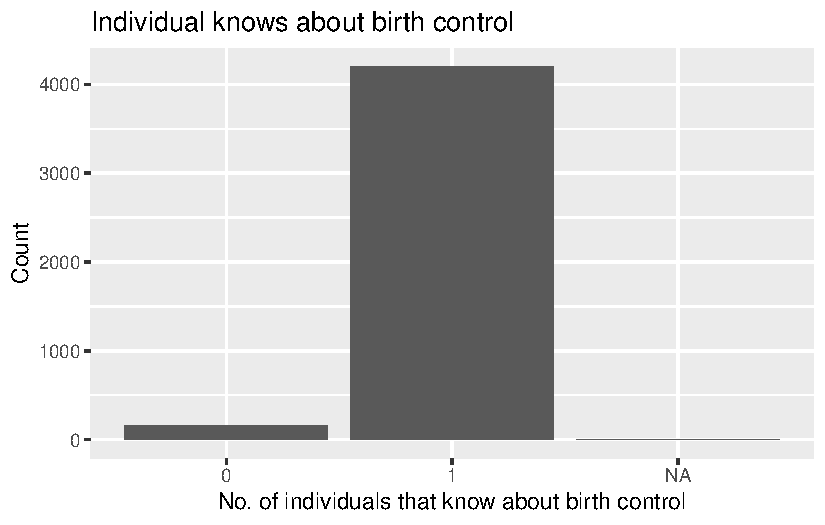
\includegraphics{Fertility_Rates_Education_Impact_Botswana_files/figure-pdf/unnamed-chunk-23-1.pdf}

}

\end{figure}

Here, we can see that most individuals know about birth control.

\begin{Shaded}
\begin{Highlighting}[]
\FunctionTok{ggplot}\NormalTok{(}\AttributeTok{data =}\NormalTok{ Womendata,}
       \FunctionTok{aes}\NormalTok{(}
         \AttributeTok{x =}\NormalTok{ children,}
         \AttributeTok{y =} \FunctionTok{prop.table}\NormalTok{(}\FunctionTok{stat}\NormalTok{(count)),}
         \AttributeTok{fill =} \FunctionTok{factor}\NormalTok{(usemeth), }\AttributeTok{width =} \DecValTok{1}\NormalTok{,}
         \AttributeTok{label =}\NormalTok{ scales}\SpecialCharTok{::}\FunctionTok{percent}\NormalTok{(}\FunctionTok{prop.table}\NormalTok{(}\FunctionTok{stat}\NormalTok{(count)))}
\NormalTok{       )) }\SpecialCharTok{+}
  \FunctionTok{geom\_bar}\NormalTok{(}\AttributeTok{position =} \FunctionTok{position\_dodge}\NormalTok{()) }\SpecialCharTok{+}
  \FunctionTok{geom\_text}\NormalTok{(}
    \AttributeTok{stat =} \StringTok{"count"}\NormalTok{,}
    \AttributeTok{position =} \FunctionTok{position\_dodge}\NormalTok{(}\FloatTok{0.2}\NormalTok{),}
    \AttributeTok{vjust =} \SpecialCharTok{{-}}\DecValTok{1}\NormalTok{,}
    \AttributeTok{size =} \FloatTok{1.5}
\NormalTok{  ) }\SpecialCharTok{+} \FunctionTok{scale\_y\_continuous}\NormalTok{(}\AttributeTok{labels =}\NormalTok{ scales}\SpecialCharTok{::}\NormalTok{percent) }\SpecialCharTok{+}
  \FunctionTok{labs}\NormalTok{(}\AttributeTok{title =} \StringTok{"Number of children based on birth control"}\NormalTok{,}
       \AttributeTok{x =} \StringTok{"Number of Children"}\NormalTok{,}
       \AttributeTok{y =} \StringTok{"Count"}\NormalTok{) }\SpecialCharTok{+}
  \FunctionTok{theme\_classic}\NormalTok{() }\SpecialCharTok{+}
  \FunctionTok{scale\_fill\_discrete}\NormalTok{(}
    \AttributeTok{name =} \StringTok{"Birth Control"}\NormalTok{,}
    \AttributeTok{labels =} \FunctionTok{c}\NormalTok{(}\StringTok{"Use birth control"}\NormalTok{, }\StringTok{"Never used birth control"}\NormalTok{)}
\NormalTok{  )}
\end{Highlighting}
\end{Shaded}

\begin{verbatim}
Warning: `stat(count)` was deprecated in ggplot2 3.4.0.
i Please use `after_stat(count)` instead.
\end{verbatim}

\begin{figure}[H]

{\centering 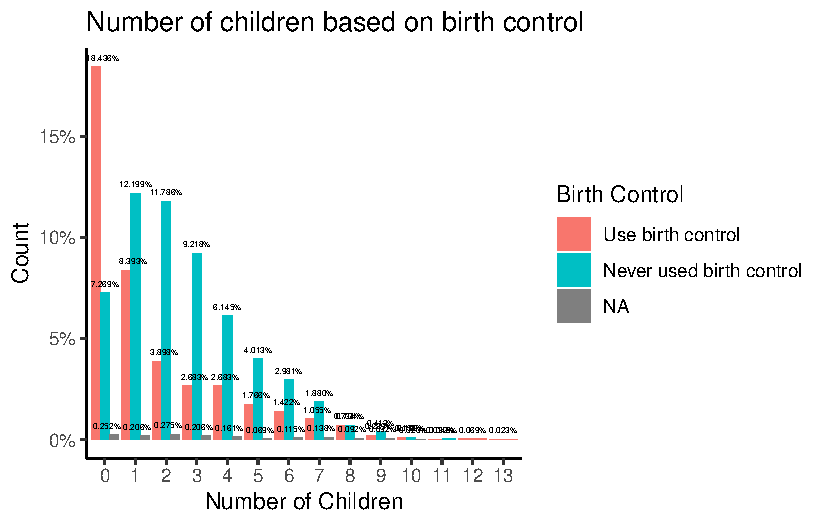
\includegraphics{Fertility_Rates_Education_Impact_Botswana_files/figure-pdf/unnamed-chunk-24-1.pdf}

}

\end{figure}

Here we can see that the number of individuals using birth control is
higher than individuals that never used birth control only for
individuals have zero children. As the number of children go up we can
see that individuals most individuals that have never used birth control
are higher than the indivuals that have used birth control. This can
imply that the percentage individuals that have children and use birth
control are lesser than the percentage individuals that have children
and never used birth control.

\begin{Shaded}
\begin{Highlighting}[]
\FunctionTok{ggplot}\NormalTok{(Womendatacleaned,}\FunctionTok{aes}\NormalTok{(}\AttributeTok{x=}\FunctionTok{factor}\NormalTok{(children),}\AttributeTok{fill=}\FunctionTok{factor}\NormalTok{(evermarr)))}\SpecialCharTok{+}
  
\FunctionTok{geom\_bar}\NormalTok{()}\SpecialCharTok{+}\FunctionTok{theme}\NormalTok{(}\AttributeTok{axis.text.x =} \FunctionTok{element\_text}\NormalTok{(}\AttributeTok{face=}\StringTok{"bold"}\NormalTok{, }\AttributeTok{size=}\DecValTok{15}\NormalTok{),}\AttributeTok{axis.text.y =} \FunctionTok{element\_text}\NormalTok{(}\AttributeTok{face=}\StringTok{"bold"}\NormalTok{, }\AttributeTok{size=}\DecValTok{15}\NormalTok{))}\SpecialCharTok{+}
  
\FunctionTok{labs}\NormalTok{(}
    \AttributeTok{title =} \StringTok{"Number of Children based on Marriage status"}\NormalTok{,}
    \AttributeTok{x =} \StringTok{"Number of children"}\NormalTok{,}
    \AttributeTok{y =} \StringTok{"Count"}\NormalTok{,}\AttributeTok{size=}\DecValTok{15}\NormalTok{) }\SpecialCharTok{+}
   
\FunctionTok{scale\_fill\_manual}\NormalTok{(}
    \AttributeTok{name =} \StringTok{"Married or not"}\NormalTok{,}
    \AttributeTok{breaks =} \FunctionTok{c}\NormalTok{(}\StringTok{"0"}\NormalTok{, }\StringTok{"1"}\NormalTok{),}
    \AttributeTok{labels =} \FunctionTok{c}\NormalTok{(}\StringTok{"Not Married"}\NormalTok{, }\StringTok{"Married"}\NormalTok{),}
    \AttributeTok{values =} \FunctionTok{c}\NormalTok{(}\StringTok{"0"} \OtherTok{=} \StringTok{"blue"}\NormalTok{, }\StringTok{"1"}\OtherTok{=}\StringTok{"red"}\NormalTok{)}
\NormalTok{  )}
\end{Highlighting}
\end{Shaded}

\begin{figure}[H]

{\centering 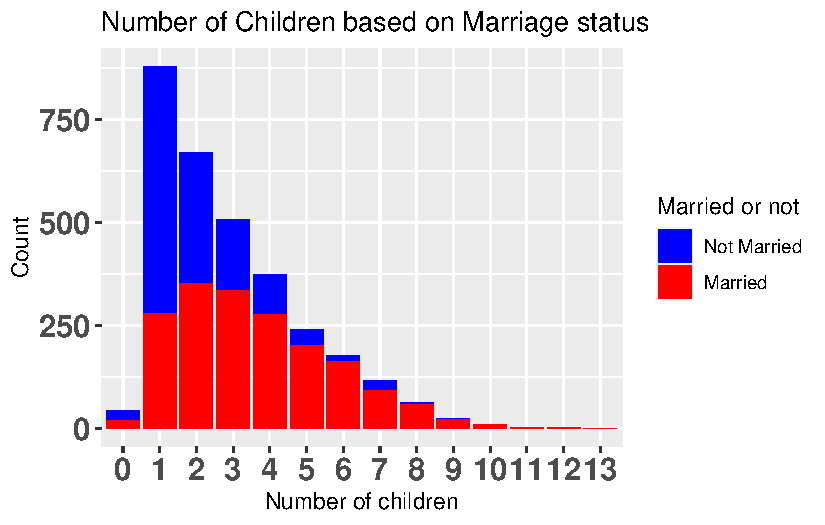
\includegraphics{Fertility_Rates_Education_Impact_Botswana_files/figure-pdf/unnamed-chunk-25-1.pdf}

}

\end{figure}

Most women have 1 child in majority. Majority of those mothers are not
married. This could say something about our data.

\begin{Shaded}
\begin{Highlighting}[]
\NormalTok{Womendata }\SpecialCharTok{\%\textgreater{}\%}
  \FunctionTok{ggplot}\NormalTok{() }\SpecialCharTok{+}
  \FunctionTok{geom\_bar}\NormalTok{(}\FunctionTok{aes}\NormalTok{(educ)) }\SpecialCharTok{+}
  \FunctionTok{theme\_classic}\NormalTok{() }\SpecialCharTok{+} \FunctionTok{labs}\NormalTok{(}\AttributeTok{title =} \StringTok{"Number of children based on years of schooling"}\NormalTok{,}
       \AttributeTok{x =} \StringTok{"Number of years of schooling"}\NormalTok{,}
       \AttributeTok{y =} \StringTok{"Count"}\NormalTok{)}
\end{Highlighting}
\end{Shaded}

\begin{figure}[H]

{\centering 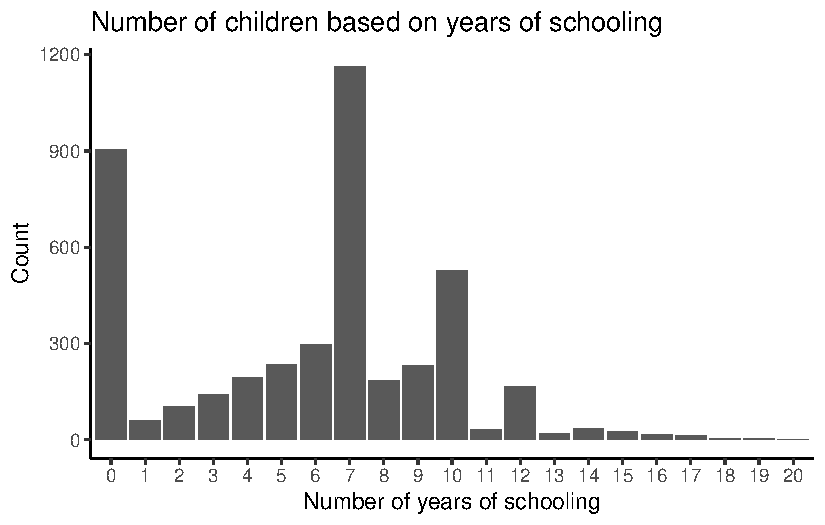
\includegraphics{Fertility_Rates_Education_Impact_Botswana_files/figure-pdf/unnamed-chunk-26-1.pdf}

}

\end{figure}

\begin{Shaded}
\begin{Highlighting}[]
  \FunctionTok{ggtitle}\NormalTok{(}\StringTok{"No of indviduals educated"}\NormalTok{)}
\end{Highlighting}
\end{Shaded}

\begin{verbatim}
$title
[1] "No of indviduals educated"

attr(,"class")
[1] "labels"
\end{verbatim}

From the bar graph we can say that majority of women in our data have
education of atleast 5-7 years and the next highest is women with 0
years of education. This can say a lot about our data when we are
talking about the relationship between education and fertility.

\begin{Shaded}
\begin{Highlighting}[]
\FunctionTok{ggplot}\NormalTok{(Womendatacleaned,}\FunctionTok{aes}\NormalTok{(}\AttributeTok{x=}\FunctionTok{factor}\NormalTok{(age),}\AttributeTok{fill=}\FunctionTok{factor}\NormalTok{(usemeth)))}\SpecialCharTok{+}
  
\FunctionTok{geom\_bar}\NormalTok{()}\SpecialCharTok{+}\FunctionTok{theme}\NormalTok{(}\AttributeTok{axis.text.x =} \FunctionTok{element\_text}\NormalTok{(}\AttributeTok{face=}\StringTok{"bold"}\NormalTok{, }\AttributeTok{size=}\DecValTok{5}\NormalTok{),}\AttributeTok{axis.text.y =} \FunctionTok{element\_text}\NormalTok{(}\AttributeTok{face=}\StringTok{"bold"}\NormalTok{, }\AttributeTok{size=}\DecValTok{15}\NormalTok{))}\SpecialCharTok{+}
  
\FunctionTok{labs}\NormalTok{(}
    \AttributeTok{title =} \StringTok{"Number of individuals that have used birth control based their age"}\NormalTok{,}
    \AttributeTok{x =} \StringTok{"Age"}\NormalTok{,}
    \AttributeTok{y =} \StringTok{"Count"}\NormalTok{,}\AttributeTok{size=}\DecValTok{15}\NormalTok{) }\SpecialCharTok{+}
   
\FunctionTok{scale\_fill\_manual}\NormalTok{(}
    \AttributeTok{name =} \StringTok{"Use birth control or not"}\NormalTok{,}
    \AttributeTok{breaks =} \FunctionTok{c}\NormalTok{(}\StringTok{"0"}\NormalTok{, }\StringTok{"1"}\NormalTok{),}
    \AttributeTok{labels =} \FunctionTok{c}\NormalTok{(}\StringTok{"Never used birth control"}\NormalTok{, }\StringTok{"Has used birth control"}\NormalTok{),}
    \AttributeTok{values =} \FunctionTok{c}\NormalTok{(}\StringTok{"0"} \OtherTok{=} \StringTok{"brown"}\NormalTok{, }\StringTok{"1"}\OtherTok{=}\StringTok{"green"}\NormalTok{)}
\NormalTok{  )}
\end{Highlighting}
\end{Shaded}

\begin{figure}[H]

{\centering 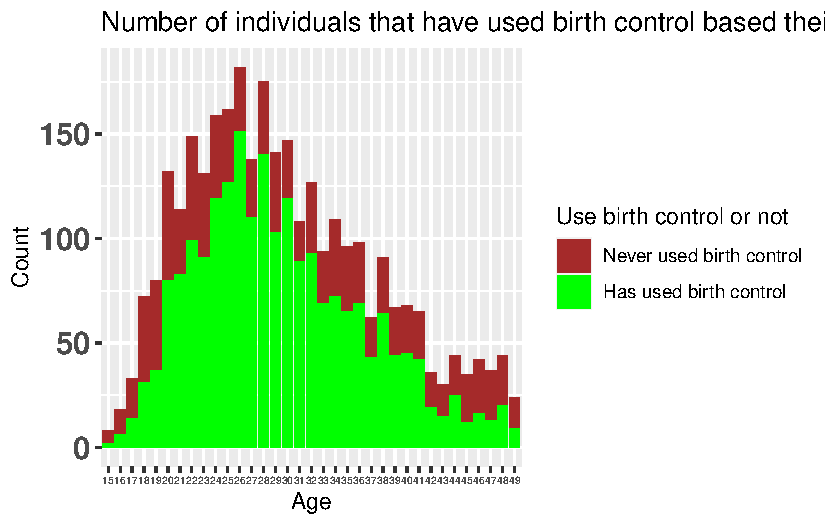
\includegraphics{Fertility_Rates_Education_Impact_Botswana_files/figure-pdf/unnamed-chunk-27-1.pdf}

}

\end{figure}

\begin{Shaded}
\begin{Highlighting}[]
\FunctionTok{ggplot}\NormalTok{(}\AttributeTok{data =}\NormalTok{ Womendata, }\FunctionTok{aes}\NormalTok{(}\AttributeTok{x=}\NormalTok{mnthborn, }\AttributeTok{y=}\NormalTok{ children)) }\SpecialCharTok{+} 
  \FunctionTok{geom\_boxplot}\NormalTok{(}\AttributeTok{outlier.color =} \StringTok{"red"}\NormalTok{, }\AttributeTok{outlier.shape =} \DecValTok{1}\NormalTok{, }\AttributeTok{show.legend =}\NormalTok{ T) }\SpecialCharTok{+} 
  \FunctionTok{facet\_wrap}\NormalTok{(}\SpecialCharTok{\textasciitilde{}}\NormalTok{mnthborn)}
\end{Highlighting}
\end{Shaded}

\begin{figure}[H]

{\centering 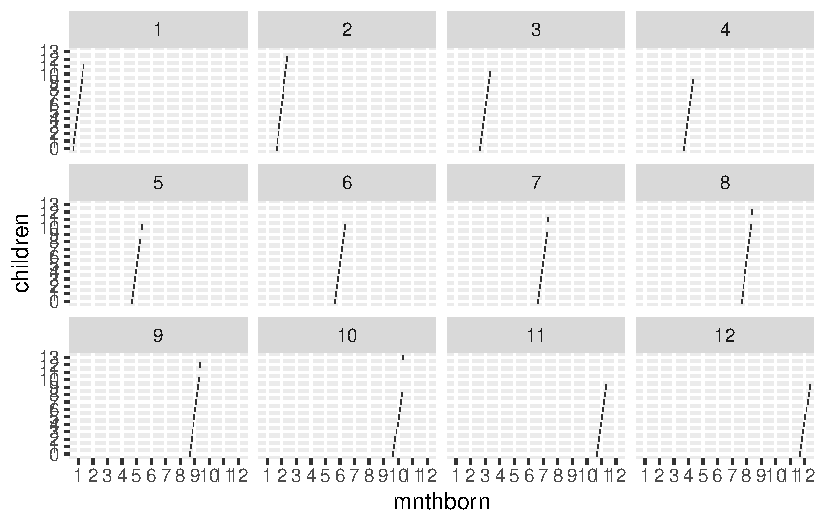
\includegraphics{Fertility_Rates_Education_Impact_Botswana_files/figure-pdf/unnamed-chunk-28-1.pdf}

}

\end{figure}

\begin{Shaded}
\begin{Highlighting}[]
\FunctionTok{ggplot}\NormalTok{(}\AttributeTok{data =}\NormalTok{ Womendata) }\SpecialCharTok{+} 
  \FunctionTok{geom\_violin}\NormalTok{(}\AttributeTok{mapping =} \FunctionTok{aes}\NormalTok{(}\AttributeTok{y=}\NormalTok{children, }\AttributeTok{x =}\NormalTok{ educ,}\AttributeTok{fill=}\NormalTok{educ), }\AttributeTok{trim =} \ConstantTok{TRUE}\NormalTok{, }\AttributeTok{draw\_quantiles =} \FunctionTok{c}\NormalTok{(}\FloatTok{0.25}\NormalTok{, }\FloatTok{0.5}\NormalTok{, }\FloatTok{0.75}\NormalTok{))}
\end{Highlighting}
\end{Shaded}

\begin{verbatim}
Warning: Groups with fewer than two data points have been dropped.
Groups with fewer than two data points have been dropped.
Groups with fewer than two data points have been dropped.
Groups with fewer than two data points have been dropped.
Groups with fewer than two data points have been dropped.
Groups with fewer than two data points have been dropped.
Groups with fewer than two data points have been dropped.
Groups with fewer than two data points have been dropped.
Groups with fewer than two data points have been dropped.
Groups with fewer than two data points have been dropped.
Groups with fewer than two data points have been dropped.
Groups with fewer than two data points have been dropped.
Groups with fewer than two data points have been dropped.
Groups with fewer than two data points have been dropped.
Groups with fewer than two data points have been dropped.
Groups with fewer than two data points have been dropped.
Groups with fewer than two data points have been dropped.
Groups with fewer than two data points have been dropped.
Groups with fewer than two data points have been dropped.
Groups with fewer than two data points have been dropped.
Groups with fewer than two data points have been dropped.
Groups with fewer than two data points have been dropped.
Groups with fewer than two data points have been dropped.
Groups with fewer than two data points have been dropped.
Groups with fewer than two data points have been dropped.
Groups with fewer than two data points have been dropped.
\end{verbatim}

\begin{figure}[H]

{\centering 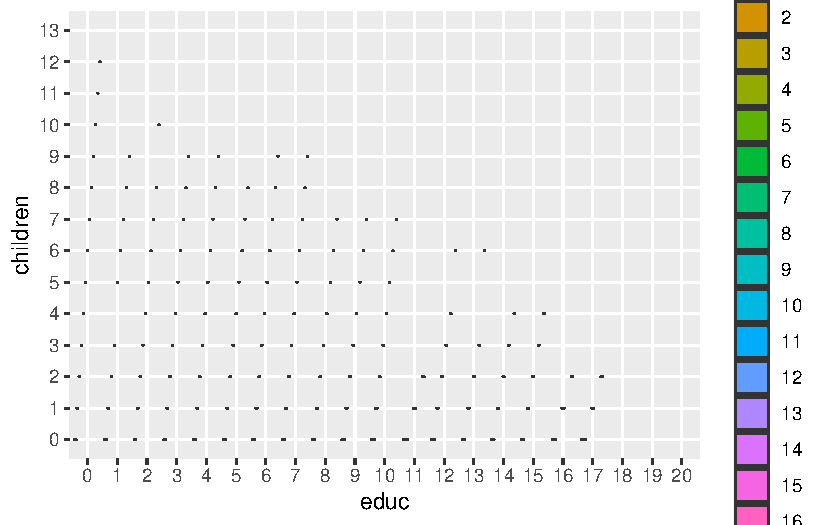
\includegraphics{Fertility_Rates_Education_Impact_Botswana_files/figure-pdf/unnamed-chunk-29-1.pdf}

}

\end{figure}

\begin{Shaded}
\begin{Highlighting}[]
\FunctionTok{plot\_bar}\NormalTok{(}\AttributeTok{data =}\NormalTok{ Womendata)}
\end{Highlighting}
\end{Shaded}

\begin{figure}[H]

{\centering 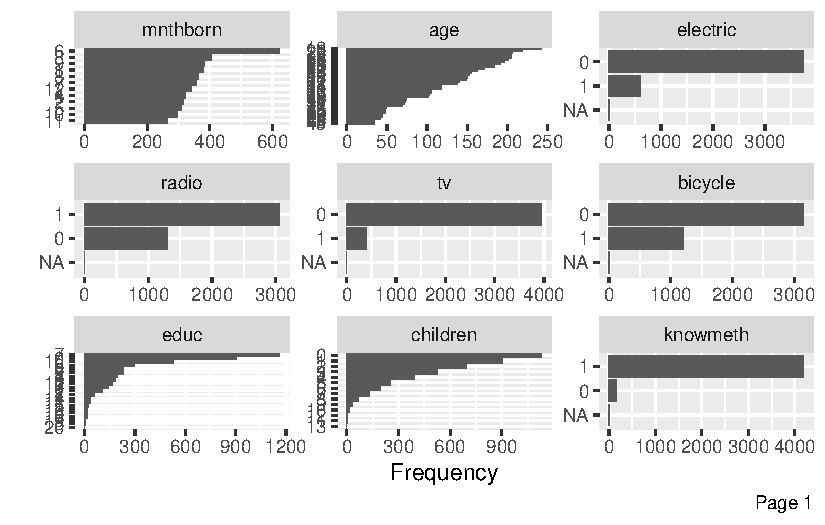
\includegraphics{Fertility_Rates_Education_Impact_Botswana_files/figure-pdf/unnamed-chunk-30-1.pdf}

}

\end{figure}

\begin{figure}[H]

{\centering 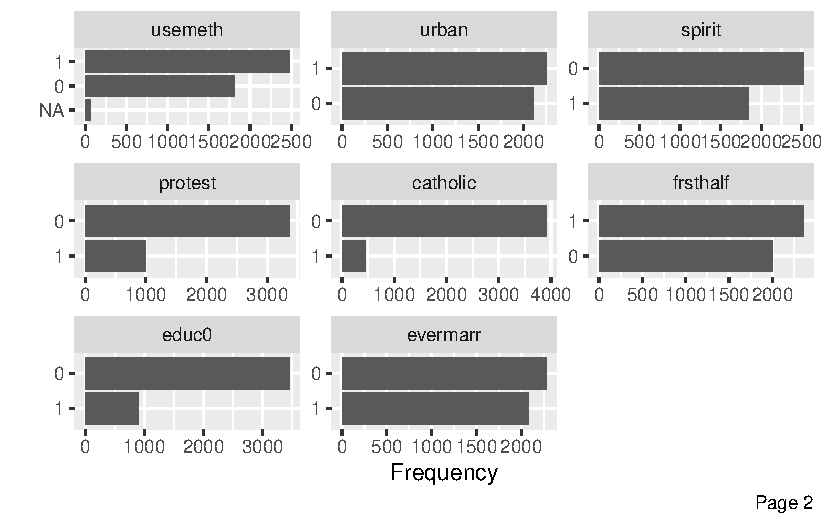
\includegraphics{Fertility_Rates_Education_Impact_Botswana_files/figure-pdf/unnamed-chunk-30-2.pdf}

}

\end{figure}

\begin{Shaded}
\begin{Highlighting}[]
\NormalTok{Womendata}\SpecialCharTok{$}\NormalTok{educ }\OtherTok{\textless{}{-}}\FunctionTok{as.integer}\NormalTok{(}\FunctionTok{as.character}\NormalTok{(Womendata}\SpecialCharTok{$}\NormalTok{educ))}
\NormalTok{Womendata}\SpecialCharTok{$}\NormalTok{age }\OtherTok{\textless{}{-}} \FunctionTok{as.integer}\NormalTok{(}\FunctionTok{as.character}\NormalTok{(Womendata}\SpecialCharTok{$}\NormalTok{age))}

\NormalTok{Womendata}\SpecialCharTok{$}\NormalTok{mnthborn }\OtherTok{\textless{}{-}} \FunctionTok{as.integer}\NormalTok{(}\FunctionTok{as.character}\NormalTok{(Womendata}\SpecialCharTok{$}\NormalTok{mnthborn))}
\NormalTok{Womendata}\SpecialCharTok{$}\NormalTok{electric }\OtherTok{\textless{}{-}} \FunctionTok{as.integer}\NormalTok{(}\FunctionTok{as.character}\NormalTok{(Womendata}\SpecialCharTok{$}\NormalTok{electric))}

\NormalTok{Womendata}\SpecialCharTok{$}\NormalTok{radio }\OtherTok{\textless{}{-}} \FunctionTok{as.integer}\NormalTok{(}\FunctionTok{as.character}\NormalTok{(Womendata}\SpecialCharTok{$}\NormalTok{radio))}
\NormalTok{Womendata}\SpecialCharTok{$}\NormalTok{tv }\OtherTok{\textless{}{-}} \FunctionTok{as.integer}\NormalTok{(}\FunctionTok{as.character}\NormalTok{(Womendata}\SpecialCharTok{$}\NormalTok{tv))}

\NormalTok{Womendata}\SpecialCharTok{$}\NormalTok{bicycle }\OtherTok{\textless{}{-}} \FunctionTok{as.integer}\NormalTok{(}\FunctionTok{as.character}\NormalTok{(Womendata}\SpecialCharTok{$}\NormalTok{bicycle))}
\NormalTok{Womendata}\SpecialCharTok{$}\NormalTok{children }\OtherTok{\textless{}{-}} \FunctionTok{as.integer}\NormalTok{(}\FunctionTok{as.character}\NormalTok{(Womendata}\SpecialCharTok{$}\NormalTok{children))}

\NormalTok{Womendata}\SpecialCharTok{$}\NormalTok{knowmeth }\OtherTok{\textless{}{-}} \FunctionTok{as.integer}\NormalTok{(}\FunctionTok{as.character}\NormalTok{(Womendata}\SpecialCharTok{$}\NormalTok{knowmeth))}
\FunctionTok{plot\_histogram}\NormalTok{(}\AttributeTok{data =}\NormalTok{ Womendata)}
\end{Highlighting}
\end{Shaded}

\begin{figure}[H]

{\centering 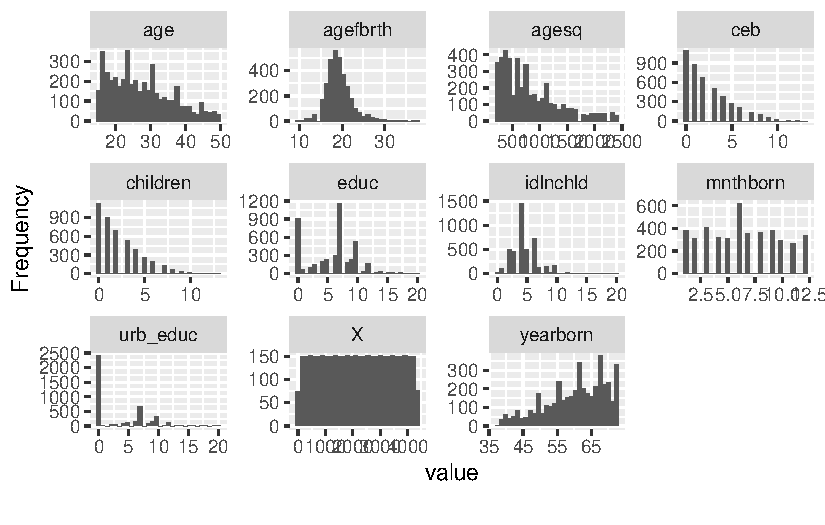
\includegraphics{Fertility_Rates_Education_Impact_Botswana_files/figure-pdf/unnamed-chunk-31-1.pdf}

}

\end{figure}

\hypertarget{corelation}{%
\subsection{Corelation}\label{corelation}}

\begin{Shaded}
\begin{Highlighting}[]
\FunctionTok{library}\NormalTok{(corrplot)}
\end{Highlighting}
\end{Shaded}

\begin{verbatim}
corrplot 0.92 loaded
\end{verbatim}

\begin{Shaded}
\begin{Highlighting}[]
\FunctionTok{library}\NormalTok{(RColorBrewer)}

\NormalTok{M }\OtherTok{\textless{}{-}}\FunctionTok{cor}\NormalTok{(Womendata }\SpecialCharTok{\%\textgreater{}\%} 
\NormalTok{         dplyr}\SpecialCharTok{::}\FunctionTok{select}\NormalTok{(age, yearborn, educ, ceb, agefbrth, children, usemeth, knowmeth))}

\FunctionTok{corrplot}\NormalTok{(M, }\AttributeTok{type=}\StringTok{"upper"}\NormalTok{, }\AttributeTok{order =} \StringTok{"original"}\NormalTok{,}\AttributeTok{col=}\FunctionTok{brewer.pal}\NormalTok{(}\AttributeTok{n=}\DecValTok{8}\NormalTok{, }\AttributeTok{name=}\StringTok{"RdYlBu"}\NormalTok{))}
\end{Highlighting}
\end{Shaded}

\begin{figure}[H]

{\centering 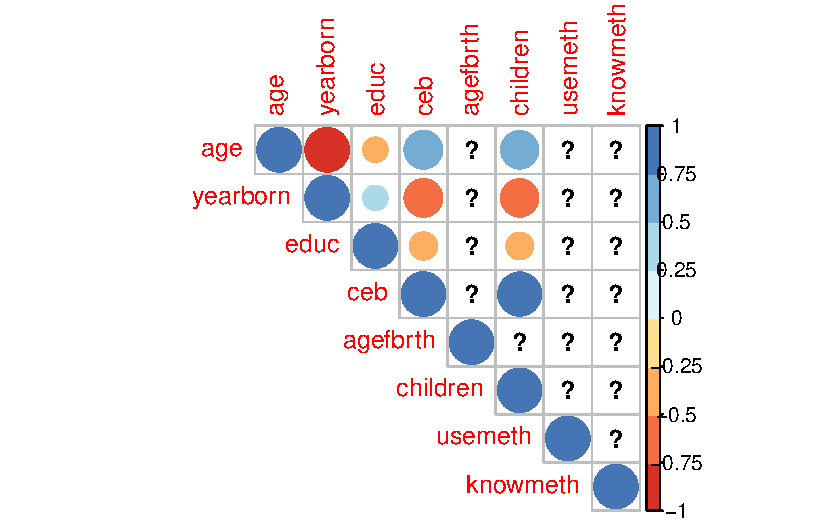
\includegraphics{Fertility_Rates_Education_Impact_Botswana_files/figure-pdf/unnamed-chunk-32-1.pdf}

}

\end{figure}

\begin{Shaded}
\begin{Highlighting}[]
\FunctionTok{cor}\NormalTok{(Womendata}\SpecialCharTok{$}\NormalTok{educ, Womendata}\SpecialCharTok{$}\NormalTok{children)}
\end{Highlighting}
\end{Shaded}

\begin{verbatim}
[1] -0.3705226
\end{verbatim}

Here we can see that education and number of children have a negative
correlation. Negative correlation is a relationship between two
variables in which one variable increases as the other decreases, and
vice versa.

\begin{Shaded}
\begin{Highlighting}[]
\FunctionTok{cor}\NormalTok{(Womendata}\SpecialCharTok{$}\NormalTok{educ, Womendata}\SpecialCharTok{$}\NormalTok{ceb)}
\end{Highlighting}
\end{Shaded}

\begin{verbatim}
[1] -0.3842877
\end{verbatim}

Here we can see that education and number of children ever born have a
negative correlation as well. This does say lot about education and
number of children.

\begin{Shaded}
\begin{Highlighting}[]
\FunctionTok{cor}\NormalTok{(Womendata}\SpecialCharTok{$}\NormalTok{age, }\FunctionTok{unclass}\NormalTok{(Womendata}\SpecialCharTok{$}\NormalTok{educ))}
\end{Highlighting}
\end{Shaded}

\begin{verbatim}
[1] -0.3096017
\end{verbatim}

We can see that age and education have a negative correlation.

\begin{Shaded}
\begin{Highlighting}[]
\FunctionTok{cor}\NormalTok{(Womendata}\SpecialCharTok{$}\NormalTok{age, Womendata}\SpecialCharTok{$}\NormalTok{children)}
\end{Highlighting}
\end{Shaded}

\begin{verbatim}
[1] 0.7325709
\end{verbatim}

Age and number of children have a positive correlation.

\begin{Shaded}
\begin{Highlighting}[]
\FunctionTok{library}\NormalTok{(PerformanceAnalytics)}
\end{Highlighting}
\end{Shaded}

\begin{verbatim}
Loading required package: xts
\end{verbatim}

\begin{verbatim}

######################### Warning from 'xts' package ##########################
#                                                                             #
# The dplyr lag() function breaks how base R's lag() function is supposed to  #
# work, which breaks lag(my_xts). Calls to lag(my_xts) that you type or       #
# source() into this session won't work correctly.                            #
#                                                                             #
# Use stats::lag() to make sure you're not using dplyr::lag(), or you can add #
# conflictRules('dplyr', exclude = 'lag') to your .Rprofile to stop           #
# dplyr from breaking base R's lag() function.                                #
#                                                                             #
# Code in packages is not affected. It's protected by R's namespace mechanism #
# Set `options(xts.warn_dplyr_breaks_lag = FALSE)` to suppress this warning.  #
#                                                                             #
###############################################################################
\end{verbatim}

\begin{verbatim}

Attaching package: 'xts'
\end{verbatim}

\begin{verbatim}
The following objects are masked from 'package:dplyr':

    first, last
\end{verbatim}

\begin{verbatim}

Attaching package: 'PerformanceAnalytics'
\end{verbatim}

\begin{verbatim}
The following object is masked from 'package:graphics':

    legend
\end{verbatim}

\begin{Shaded}
\begin{Highlighting}[]
\FunctionTok{chart.Correlation}\NormalTok{(Womendata }\SpecialCharTok{\%\textgreater{}\%} 
\NormalTok{              dplyr}\SpecialCharTok{::}\FunctionTok{select}\NormalTok{(age,yearborn, educ, ceb, agefbrth, children), }\AttributeTok{histogram=}\ConstantTok{TRUE}\NormalTok{, }\AttributeTok{pch=}\DecValTok{19}\NormalTok{)}
\end{Highlighting}
\end{Shaded}

\begin{verbatim}
Warning in par(usr): argument 1 does not name a graphical parameter

Warning in par(usr): argument 1 does not name a graphical parameter

Warning in par(usr): argument 1 does not name a graphical parameter

Warning in par(usr): argument 1 does not name a graphical parameter

Warning in par(usr): argument 1 does not name a graphical parameter

Warning in par(usr): argument 1 does not name a graphical parameter

Warning in par(usr): argument 1 does not name a graphical parameter

Warning in par(usr): argument 1 does not name a graphical parameter

Warning in par(usr): argument 1 does not name a graphical parameter

Warning in par(usr): argument 1 does not name a graphical parameter

Warning in par(usr): argument 1 does not name a graphical parameter

Warning in par(usr): argument 1 does not name a graphical parameter

Warning in par(usr): argument 1 does not name a graphical parameter

Warning in par(usr): argument 1 does not name a graphical parameter

Warning in par(usr): argument 1 does not name a graphical parameter
\end{verbatim}

\begin{figure}[H]

{\centering 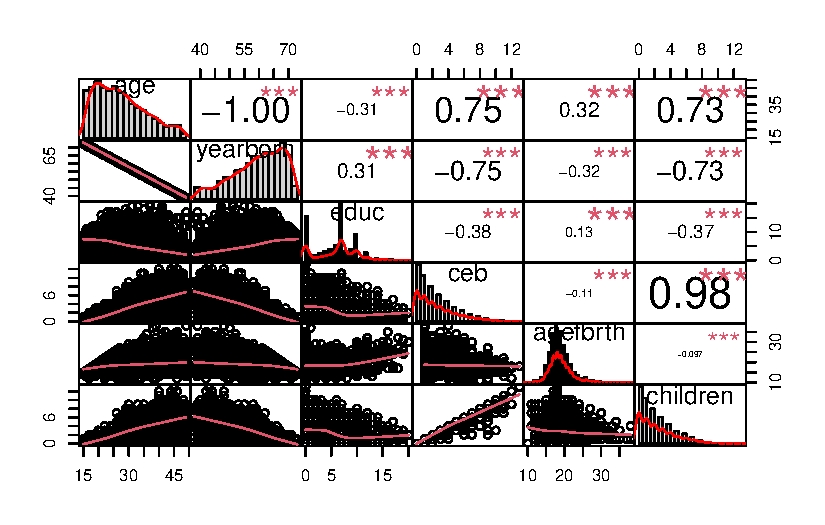
\includegraphics{Fertility_Rates_Education_Impact_Botswana_files/figure-pdf/unnamed-chunk-37-1.pdf}

}

\end{figure}

\begin{Shaded}
\begin{Highlighting}[]
\NormalTok{Womendata}\SpecialCharTok{$}\NormalTok{educ }\OtherTok{\textless{}{-}} \FunctionTok{as.factor}\NormalTok{(Womendata}\SpecialCharTok{$}\NormalTok{educ)}
\NormalTok{Womendata}\SpecialCharTok{$}\NormalTok{age }\OtherTok{\textless{}{-}} \FunctionTok{as.factor}\NormalTok{(Womendata}\SpecialCharTok{$}\NormalTok{age)}

\NormalTok{Womendata}\SpecialCharTok{$}\NormalTok{mnthborn }\OtherTok{\textless{}{-}} \FunctionTok{as.factor}\NormalTok{(Womendata}\SpecialCharTok{$}\NormalTok{mnthborn)}
\NormalTok{Womendata}\SpecialCharTok{$}\NormalTok{electric }\OtherTok{\textless{}{-}} \FunctionTok{as.factor}\NormalTok{(Womendata}\SpecialCharTok{$}\NormalTok{electric)}

\NormalTok{Womendata}\SpecialCharTok{$}\NormalTok{radio }\OtherTok{\textless{}{-}} \FunctionTok{as.factor}\NormalTok{(Womendata}\SpecialCharTok{$}\NormalTok{radio)}
\NormalTok{Womendata}\SpecialCharTok{$}\NormalTok{tv }\OtherTok{\textless{}{-}} \FunctionTok{as.factor}\NormalTok{(Womendata}\SpecialCharTok{$}\NormalTok{tv)}

\NormalTok{Womendata}\SpecialCharTok{$}\NormalTok{bicycle }\OtherTok{\textless{}{-}} \FunctionTok{as.factor}\NormalTok{(Womendata}\SpecialCharTok{$}\NormalTok{bicycle)}
\NormalTok{Womendata}\SpecialCharTok{$}\NormalTok{children }\OtherTok{\textless{}{-}} \FunctionTok{as.factor}\NormalTok{(Womendata}\SpecialCharTok{$}\NormalTok{children)}

\NormalTok{Womendata}\SpecialCharTok{$}\NormalTok{knowmeth }\OtherTok{\textless{}{-}} \FunctionTok{as.factor}\NormalTok{(Womendata}\SpecialCharTok{$}\NormalTok{knowmeth)}
\NormalTok{Womendata}\SpecialCharTok{$}\NormalTok{catholic }\OtherTok{\textless{}{-}} \FunctionTok{as.factor}\NormalTok{(Womendata}\SpecialCharTok{$}\NormalTok{catholic)}

\NormalTok{Womendata}\SpecialCharTok{$}\NormalTok{frsthalf }\OtherTok{\textless{}{-}} \FunctionTok{as.factor}\NormalTok{(Womendata}\SpecialCharTok{$}\NormalTok{frsthalf)}
\NormalTok{Womendata}\SpecialCharTok{$}\NormalTok{educ0 }\OtherTok{\textless{}{-}} \FunctionTok{as.factor}\NormalTok{(Womendata}\SpecialCharTok{$}\NormalTok{educ0)}

\NormalTok{Womendata}\SpecialCharTok{$}\NormalTok{evermarr }\OtherTok{\textless{}{-}} \FunctionTok{as.factor}\NormalTok{(Womendata}\SpecialCharTok{$}\NormalTok{evermarr)}
\NormalTok{Womendata}\SpecialCharTok{$}\NormalTok{protest }\OtherTok{\textless{}{-}} \FunctionTok{as.factor}\NormalTok{(Womendata}\SpecialCharTok{$}\NormalTok{protest)}
\NormalTok{Womendata}\SpecialCharTok{$}\NormalTok{spirit }\OtherTok{\textless{}{-}} \FunctionTok{as.factor}\NormalTok{(Womendata}\SpecialCharTok{$}\NormalTok{spirit)}

\NormalTok{Womendata}\SpecialCharTok{$}\NormalTok{urban }\OtherTok{\textless{}{-}} \FunctionTok{as.factor}\NormalTok{(Womendata}\SpecialCharTok{$}\NormalTok{urban)}
\NormalTok{Womendata}\SpecialCharTok{$}\NormalTok{spirit }\OtherTok{\textless{}{-}} \FunctionTok{as.factor}\NormalTok{(Womendata}\SpecialCharTok{$}\NormalTok{spirit)}
\end{Highlighting}
\end{Shaded}

\begin{Shaded}
\begin{Highlighting}[]
\FunctionTok{summary}\NormalTok{(Womendata)}
\end{Highlighting}
\end{Shaded}

\begin{verbatim}
       X           mnthborn       yearborn          age       electric   
 Min.   :   1   6      : 623   Min.   :38.00   18     : 243   0   :3747  
 1st Qu.:1091   3      : 406   1st Qu.:55.00   20     : 219   1   : 611  
 Median :2181   9      : 382   Median :62.00   22     : 206   NA's:   3  
 Mean   :2181   1      : 380   Mean   :60.43   16     : 205              
 3rd Qu.:3271   8      : 363   3rd Qu.:68.00   19     : 205              
 Max.   :4361   7      : 358   Max.   :73.00   26     : 201              
                (Other):1849                   (Other):3082              
  radio         tv       bicycle          educ           ceb        
 0   :1300   0   :3954   0   :3156   7      :1162   Min.   : 0.000  
 1   :3059   1   : 405   1   :1202   0      : 906   1st Qu.: 1.000  
 NA's:   2   NA's:   2   NA's:   3   10     : 527   Median : 2.000  
                                     6      : 298   Mean   : 2.442  
                                     5      : 234   3rd Qu.: 4.000  
                                     9      : 232   Max.   :13.000  
                                     (Other):1002                   
    agefbrth        children    knowmeth       usemeth          idlnchld     
 Min.   :10.00   0      :1132   0   : 160   Min.   :0.0000   Min.   : 0.000  
 1st Qu.:17.00   1      : 907   1   :4194   1st Qu.:0.0000   1st Qu.: 3.000  
 Median :19.00   2      : 696   NA's:   7   Median :1.0000   Median : 4.000  
 Mean   :19.01   3      : 528               Mean   :0.5776   Mean   : 4.616  
 3rd Qu.:20.00   4      : 392               3rd Qu.:1.0000   3rd Qu.: 6.000  
 Max.   :38.00   5      : 255               Max.   :1.0000   Max.   :20.000  
 NA's   :1088    (Other): 451               NA's   :71       NA's   :120     
     agesq        urban       urb_educ      spirit   protest  catholic frsthalf
 Min.   : 225.0   0:2108   Min.   : 0.000   0:2520   0:3368   0:3914   0:2004  
 1st Qu.: 400.0   1:2253   1st Qu.: 0.000   1:1841   1: 993   1: 447   1:2357  
 Median : 676.0            Median : 0.000                                      
 Mean   : 826.5            Mean   : 3.469                                      
 3rd Qu.:1089.0            3rd Qu.: 7.000                                      
 Max.   :2401.0            Max.   :20.000                                      
                                                                               
 educ0    evermarr
 0:3455   0:2282  
 1: 906   1:2079  
                  
                  
                  
                  
                  
\end{verbatim}

\begin{Shaded}
\begin{Highlighting}[]
\NormalTok{Womendata}\SpecialCharTok{$}\NormalTok{age }\OtherTok{\textless{}{-}} \FunctionTok{unclass}\NormalTok{(Womendata}\SpecialCharTok{$}\NormalTok{age)}
\NormalTok{Womendata}\SpecialCharTok{$}\NormalTok{children }\OtherTok{\textless{}{-}} \FunctionTok{unclass}\NormalTok{(Womendata}\SpecialCharTok{$}\NormalTok{children)}
\NormalTok{Womendata}\SpecialCharTok{$}\NormalTok{educ }\OtherTok{\textless{}{-}} \FunctionTok{unclass}\NormalTok{(Womendata}\SpecialCharTok{$}\NormalTok{educ)}
\end{Highlighting}
\end{Shaded}

\hypertarget{regression-models}{%
\subsection{Regression Models :}\label{regression-models}}

Multiple regression models were employed to quantify the impact of
education, age, marital status, access to utilities, and other factors
on fertility rates. The models were evaluated based on their R-squared
values, F-test significance, and multicollinearity checks.

\begin{Shaded}
\begin{Highlighting}[]
\NormalTok{model1 }\OtherTok{\textless{}{-}} \FunctionTok{lm}\NormalTok{(children }\SpecialCharTok{\textasciitilde{}}\NormalTok{ educ, }\AttributeTok{data =}\NormalTok{ Womendata)}
\FunctionTok{summary}\NormalTok{(model1)}
\end{Highlighting}
\end{Shaded}

\begin{verbatim}

Call:
lm(formula = children ~ educ, data = Womendata)

Residuals:
   Min     1Q Median     3Q    Max 
-3.495 -1.496 -0.399  1.182  9.505 

Coefficients:
            Estimate Std. Error t value Pr(>|t|)    
(Intercept)  4.70519    0.06289   74.81   <2e-16 ***
educ        -0.20965    0.00796  -26.34   <2e-16 ***
---
Signif. codes:  0 '***' 0.001 '**' 0.01 '*' 0.05 '.' 0.1 ' ' 1

Residual standard error: 2.064 on 4359 degrees of freedom
Multiple R-squared:  0.1373,    Adjusted R-squared:  0.1371 
F-statistic: 693.7 on 1 and 4359 DF,  p-value: < 2.2e-16
\end{verbatim}

\begin{Shaded}
\begin{Highlighting}[]
\NormalTok{model2 }\OtherTok{\textless{}{-}} \FunctionTok{lm}\NormalTok{(children }\SpecialCharTok{\textasciitilde{}}\NormalTok{., }\AttributeTok{data =}\NormalTok{ Womendata)}
\FunctionTok{summary}\NormalTok{(model1)}
\end{Highlighting}
\end{Shaded}

\begin{verbatim}

Call:
lm(formula = children ~ educ, data = Womendata)

Residuals:
   Min     1Q Median     3Q    Max 
-3.495 -1.496 -0.399  1.182  9.505 

Coefficients:
            Estimate Std. Error t value Pr(>|t|)    
(Intercept)  4.70519    0.06289   74.81   <2e-16 ***
educ        -0.20965    0.00796  -26.34   <2e-16 ***
---
Signif. codes:  0 '***' 0.001 '**' 0.01 '*' 0.05 '.' 0.1 ' ' 1

Residual standard error: 2.064 on 4359 degrees of freedom
Multiple R-squared:  0.1373,    Adjusted R-squared:  0.1371 
F-statistic: 693.7 on 1 and 4359 DF,  p-value: < 2.2e-16
\end{verbatim}

\begin{Shaded}
\begin{Highlighting}[]
\NormalTok{model3 }\OtherTok{\textless{}{-}} \FunctionTok{lm}\NormalTok{(children }\SpecialCharTok{\textasciitilde{}}\NormalTok{ educ }\SpecialCharTok{+}\NormalTok{ age }\SpecialCharTok{+}\NormalTok{ mnthborn }\SpecialCharTok{+}\NormalTok{ bicycle }\SpecialCharTok{+}\NormalTok{ urb\_educ }\SpecialCharTok{+}\NormalTok{ evermarr }\SpecialCharTok{+}\NormalTok{ yearborn }\SpecialCharTok{+}\NormalTok{ radio }\SpecialCharTok{+}\NormalTok{ agefbrth }\SpecialCharTok{+}\NormalTok{idlnchld }\SpecialCharTok{+}\NormalTok{ ceb, }\AttributeTok{data =}\NormalTok{ Womendata)}
\FunctionTok{summary}\NormalTok{(model3)}
\end{Highlighting}
\end{Shaded}

\begin{verbatim}

Call:
lm(formula = children ~ educ + age + mnthborn + bicycle + urb_educ + 
    evermarr + yearborn + radio + agefbrth + idlnchld + ceb, 
    data = Womendata)

Residuals:
    Min      1Q  Median      3Q     Max 
-6.0221 -0.0315  0.0745  0.2482  1.2733 

Coefficients:
              Estimate Std. Error t value Pr(>|t|)    
(Intercept) -1.0207133  3.1695672  -0.322   0.7474    
educ        -0.0001782  0.0032429  -0.055   0.9562    
age          0.0248719  0.0427747   0.581   0.5610    
mnthborn2   -0.0238081  0.0456270  -0.522   0.6018    
mnthborn3    0.0671309  0.0426656   1.573   0.1157    
mnthborn4    0.0529723  0.0451366   1.174   0.2406    
mnthborn5    0.0374369  0.0462253   0.810   0.4181    
mnthborn6    0.0572035  0.0388489   1.472   0.1410    
mnthborn7    0.0378128  0.0439550   0.860   0.3897    
mnthborn8    0.0419064  0.0450599   0.930   0.3524    
mnthborn9    0.0501796  0.0453065   1.108   0.2681    
mnthborn10   0.0197417  0.0503030   0.392   0.6947    
mnthborn11   0.0135532  0.0561693   0.241   0.8093    
mnthborn12   0.0537444  0.0613665   0.876   0.3812    
bicycle1     0.0488972  0.0211513   2.312   0.0209 *  
urb_educ     0.0019654  0.0028657   0.686   0.4929    
evermarr1    0.0428377  0.0208819   2.051   0.0403 *  
yearborn     0.0269700  0.0428099   0.630   0.5287    
radio1       0.0220766  0.0212752   1.038   0.2995    
agefbrth     0.0054808  0.0035900   1.527   0.1269    
idlnchld    -0.0083450  0.0044706  -1.867   0.0620 .  
ceb          0.9004369  0.0067066 134.262   <2e-16 ***
---
Signif. codes:  0 '***' 0.001 '**' 0.01 '*' 0.05 '.' 0.1 ' ' 1

Residual standard error: 0.5175 on 3155 degrees of freedom
  (1184 observations deleted due to missingness)
Multiple R-squared:  0.9368,    Adjusted R-squared:  0.9363 
F-statistic:  2226 on 21 and 3155 DF,  p-value: < 2.2e-16
\end{verbatim}

With an adjusted R-squared of 0.9363 model 3 best fits our data.

\begin{Shaded}
\begin{Highlighting}[]
\FunctionTok{library}\NormalTok{(MASS)}
\end{Highlighting}
\end{Shaded}

\begin{verbatim}

Attaching package: 'MASS'
\end{verbatim}

\begin{verbatim}
The following object is masked from 'package:dplyr':

    select
\end{verbatim}

\begin{Shaded}
\begin{Highlighting}[]
\NormalTok{model4}\OtherTok{\textless{}{-}} \FunctionTok{lm}\NormalTok{(}\FunctionTok{log}\NormalTok{(ceb)}\SpecialCharTok{\textasciitilde{}}\NormalTok{., }
                \AttributeTok{data =} \FunctionTok{na.omit}\NormalTok{(Womendata))}

\CommentTok{\#Using stepAIC search method for feature selection to simplify model without impacting much on the performance.}
\NormalTok{step.model }\OtherTok{\textless{}{-}} \FunctionTok{stepAIC}\NormalTok{(model4,}\AttributeTok{direction =} \StringTok{"both"}\NormalTok{,}\AttributeTok{trace =} \ConstantTok{FALSE}\NormalTok{)}

\FunctionTok{summary}\NormalTok{(step.model)}
\end{Highlighting}
\end{Shaded}

\begin{verbatim}

Call:
lm(formula = log(ceb) ~ yearborn + age + electric + radio + educ + 
    agefbrth + children + usemeth + agesq + urban + evermarr, 
    data = na.omit(Womendata))

Residuals:
     Min       1Q   Median       3Q      Max 
-1.11133 -0.14413  0.01042  0.13234  1.31158 

Coefficients:
              Estimate Std. Error t value Pr(>|t|)    
(Intercept)  2.109e+00  8.387e-01   2.515  0.01197 *  
yearborn    -2.948e-02  1.135e-02  -2.597  0.00946 ** 
age          7.227e-02  1.212e-02   5.962 2.77e-09 ***
electric1   -3.135e-02  1.330e-02  -2.357  0.01851 *  
radio1      -1.997e-02  9.531e-03  -2.096  0.03620 *  
educ        -3.248e-03  1.270e-03  -2.558  0.01059 *  
agefbrth    -2.072e-02  1.604e-03 -12.913  < 2e-16 ***
children     2.550e-01  3.157e-03  80.773  < 2e-16 ***
usemeth      4.749e-02  9.875e-03   4.809 1.59e-06 ***
agesq       -1.312e-03  6.351e-05 -20.657  < 2e-16 ***
urban1      -2.796e-02  9.072e-03  -3.083  0.00207 ** 
evermarr1    5.743e-02  9.546e-03   6.016 2.00e-09 ***
---
Signif. codes:  0 '***' 0.001 '**' 0.01 '*' 0.05 '.' 0.1 ' ' 1

Residual standard error: 0.2328 on 3106 degrees of freedom
Multiple R-squared:  0.8895,    Adjusted R-squared:  0.8891 
F-statistic:  2272 on 11 and 3106 DF,  p-value: < 2.2e-16
\end{verbatim}

\hypertarget{model-evaluation}{%
\subsection{Model Evaluation}\label{model-evaluation}}

\#\#Data Analysis: Descriptive statistics are initially employed to gain
an overview of the dataset, including measures of central tendency,
variability, and distribution of key variables. Correlation analysis is
then conducted to assess the relationships between women's education
levels, age, contraceptive use, and fertility rates. Regression models,
including linear regression and logistic regression, are utilized to
analyze the impact of education on fertility rates while controlling for
potential confounding variables such as age, marital status, and access
to healthcare.

\begin{Shaded}
\begin{Highlighting}[]
\FunctionTok{par}\NormalTok{(}\AttributeTok{mfrow=}\FunctionTok{c}\NormalTok{(}\DecValTok{2}\NormalTok{,}\DecValTok{2}\NormalTok{)) }

\FunctionTok{plot}\NormalTok{(model1)}
\end{Highlighting}
\end{Shaded}

\begin{figure}[H]

{\centering 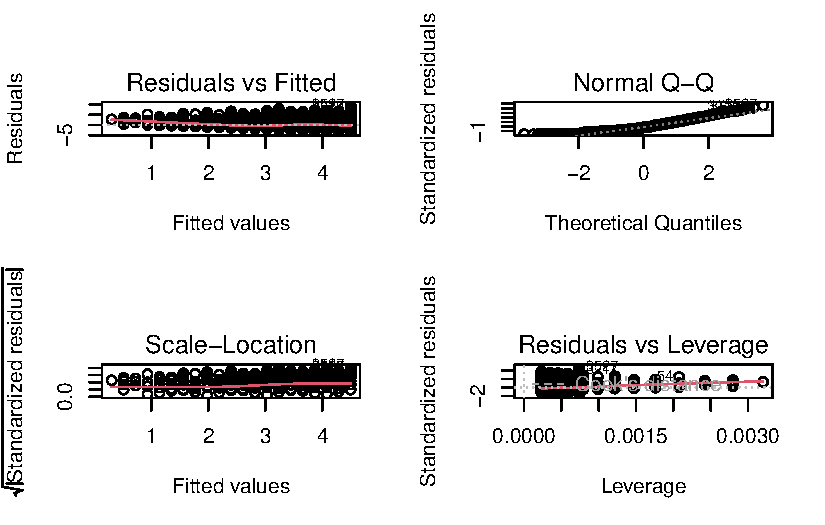
\includegraphics{Fertility_Rates_Education_Impact_Botswana_files/figure-pdf/unnamed-chunk-45-1.pdf}

}

\end{figure}

\begin{Shaded}
\begin{Highlighting}[]
\FunctionTok{par}\NormalTok{(}\AttributeTok{mfrow=}\FunctionTok{c}\NormalTok{(}\DecValTok{2}\NormalTok{,}\DecValTok{2}\NormalTok{)) }

\FunctionTok{plot}\NormalTok{(model2)}
\end{Highlighting}
\end{Shaded}

\begin{figure}[H]

{\centering 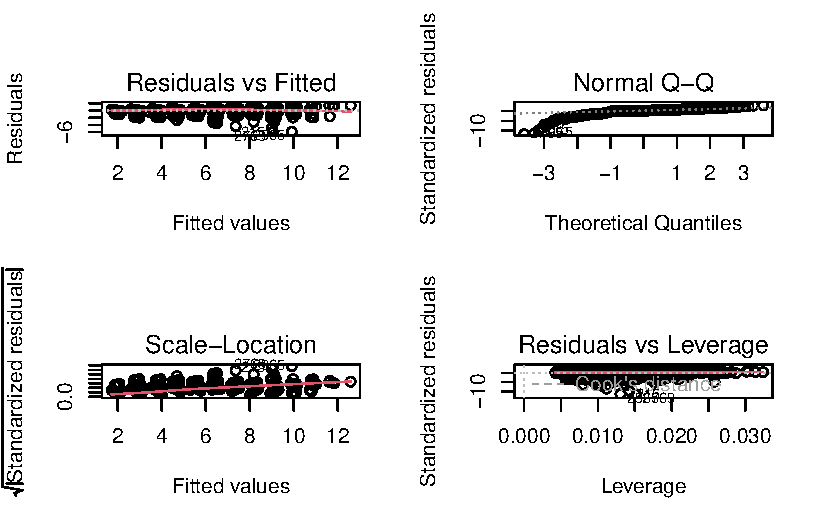
\includegraphics{Fertility_Rates_Education_Impact_Botswana_files/figure-pdf/unnamed-chunk-46-1.pdf}

}

\end{figure}

\begin{Shaded}
\begin{Highlighting}[]
\FunctionTok{par}\NormalTok{(}\AttributeTok{mfrow=}\FunctionTok{c}\NormalTok{(}\DecValTok{2}\NormalTok{,}\DecValTok{2}\NormalTok{)) }

\FunctionTok{plot}\NormalTok{(model3)}
\end{Highlighting}
\end{Shaded}

\begin{figure}[H]

{\centering 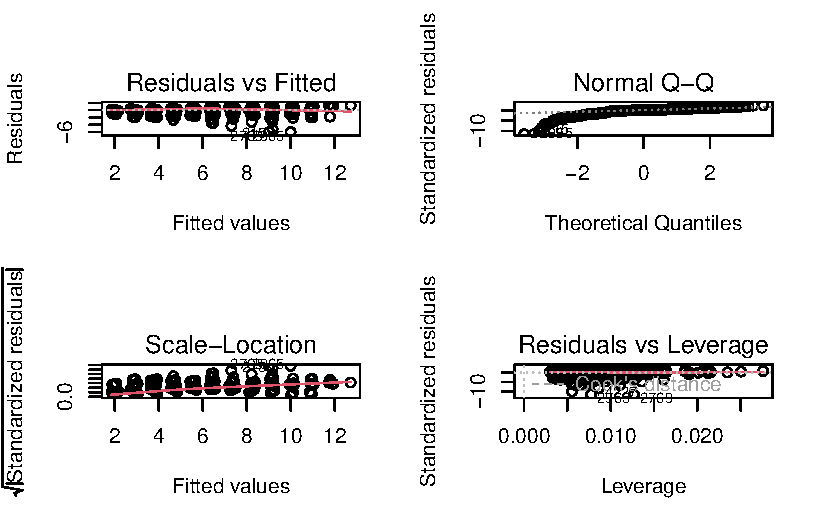
\includegraphics{Fertility_Rates_Education_Impact_Botswana_files/figure-pdf/unnamed-chunk-47-1.pdf}

}

\end{figure}

\begin{Shaded}
\begin{Highlighting}[]
\FunctionTok{par}\NormalTok{(}\AttributeTok{mfrow=}\FunctionTok{c}\NormalTok{(}\DecValTok{2}\NormalTok{,}\DecValTok{2}\NormalTok{)) }

\FunctionTok{plot}\NormalTok{(model4)}
\end{Highlighting}
\end{Shaded}

\begin{figure}[H]

{\centering 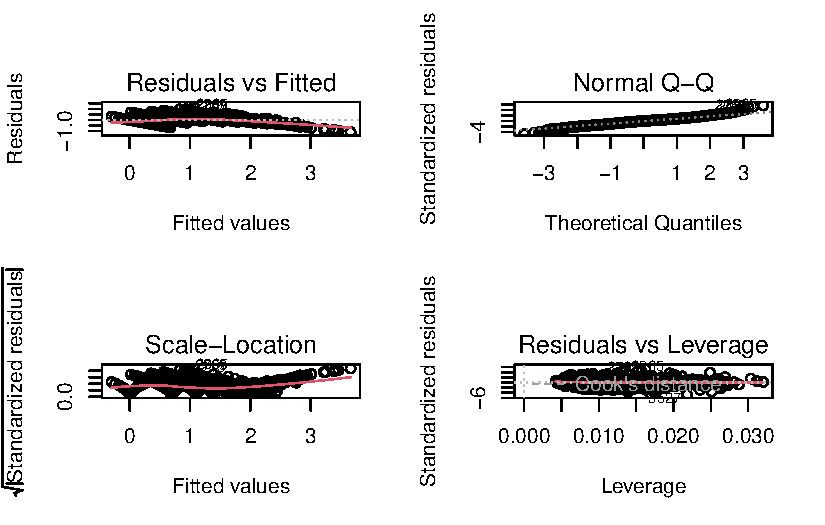
\includegraphics{Fertility_Rates_Education_Impact_Botswana_files/figure-pdf/unnamed-chunk-48-1.pdf}

}

\end{figure}

R\^{}2 = 0.8895 and adjusted R\^{}2 = 0.8891, F test value = 2272
p-value = 0.001. Under normal distribution assumption. According to
Central limit teorem , every distribution approximated by a normal
distribution. A normal distribution is approached very quickly as n
increases, note that n is the sample size for each mean and not the
number of samples If the null hypothesis is true, the above-mentioned F
test statistic can be condensed (dramatically). The test statistic will
be this sample variance ratio. If the null hypothesis is incorrect, we
will disprove both our presumption that they were equal and the null
hypothesis that the ratio was equal to 1.

\#\#Checking for Heteroskedasticity Breusch Pagan Test for
Heteroskedasticity

\begin{verbatim}
Ho: the variance is constant
H1: the variance is not constant
\end{verbatim}

\begin{Shaded}
\begin{Highlighting}[]
\FunctionTok{bptest}\NormalTok{(ceb }\SpecialCharTok{\textasciitilde{}}\NormalTok{ ., }\AttributeTok{data =}\NormalTok{ Womendatacleaned)}
\end{Highlighting}
\end{Shaded}

\begin{verbatim}

    studentized Breusch-Pagan test

data:  ceb ~ .
BP = 319.48, df = 94, p-value < 2.2e-16
\end{verbatim}

Ho hypothesis is rejected since the variance is not constant.

In multiple regression two or more predictor variables might be
correlated with each other and situation is referred as collinearity.
Multicollinearity is where collinearity exists between three or more
variables even if no pair of variables has a particularly high
correlation. This means that there is redundancy between predictor
variables.Multicollinearity can assessed by computing a score called the
variance inflation factor (or VIF), which measures how much the variance
of a regression coefficient is inflated due to multicollinearity in the
model. The smallest possible value of VIF is one (absence of
multicollinearity). A VIF value that exceeds 5 or 10 indicates a
problematic amount of collinearity.

\begin{Shaded}
\begin{Highlighting}[]
\FunctionTok{vif}\NormalTok{(step.model)}
\end{Highlighting}
\end{Shaded}

\begin{verbatim}
  yearborn        age   electric      radio       educ   agefbrth   children 
459.569426 524.025963   1.250912   1.102156   1.523564   1.430945   2.370392 
   usemeth      agesq      urban   evermarr 
  1.210953  59.396420   1.183061   1.273500 
\end{verbatim}

As a thumb rule, since we follow that a VIF value that exceeds 5 or 10
can be a problem. This leads to a simpler model without compromising the
model accuracy, which is good. So now the new model will be without
yearborn.

\hypertarget{without-multicollinearity}{%
\subsection{Without Multicollinearity}\label{without-multicollinearity}}

\begin{Shaded}
\begin{Highlighting}[]
\FunctionTok{library}\NormalTok{(MASS)}
\NormalTok{model2}\OtherTok{\textless{}{-}} \FunctionTok{lm}\NormalTok{(}\FunctionTok{log}\NormalTok{(ceb)}\SpecialCharTok{\textasciitilde{}}\NormalTok{ mnthborn }\SpecialCharTok{+}\NormalTok{ age }\SpecialCharTok{+}
\NormalTok{                            electric }\SpecialCharTok{+}
\NormalTok{                            children }\SpecialCharTok{+}\NormalTok{ knowmeth }\SpecialCharTok{+}
\NormalTok{                            usemeth  }\SpecialCharTok{+}
\NormalTok{                            urban }\SpecialCharTok{+}\NormalTok{ radio }\SpecialCharTok{+}
\NormalTok{                            tv }\SpecialCharTok{+}\NormalTok{ bicycle }\SpecialCharTok{+}
                            \FunctionTok{I}\NormalTok{(}\FunctionTok{as.factor}\NormalTok{(educ)) }\SpecialCharTok{+}
\NormalTok{                            idlnchld}\SpecialCharTok{+}\NormalTok{urb\_educ }\SpecialCharTok{+}
\NormalTok{                            protest, }
                            \AttributeTok{data =} \FunctionTok{na.omit}\NormalTok{(Womendatacleaned))}

\NormalTok{step.model2 }\OtherTok{\textless{}{-}} \FunctionTok{stepAIC}\NormalTok{(model2, }
                        \AttributeTok{direction =} \StringTok{"both"}\NormalTok{, }
                        \AttributeTok{trace =} \ConstantTok{FALSE}\NormalTok{)}

\FunctionTok{vif}\NormalTok{(step.model2) }\CommentTok{\# Variance Inflation Factor (or VIF)}
\end{Highlighting}
\end{Shaded}

\begin{verbatim}
             GVIF Df GVIF^(1/(2*Df))
age      3.298838 34        1.017707
electric 1.269286  1        1.126626
children 3.353509 13        1.047639
urban    2.365418  1        1.537992
radio    1.065265  1        1.032117
idlnchld 1.215614  1        1.102549
urb_educ 2.779986  1        1.667329
\end{verbatim}

Now the new VIF values are all less than 5. This is good for our model.
There is no Multicollinearity.

\hypertarget{key-findings}{%
\subsection{Key Findings}\label{key-findings}}

Education and Fertility: There is a clear negative correlation between
women's education levels and fertility rates. As education increases,
fertility rates tend to decrease. Birth Control Usage: Women with higher
education levels are more likely to use birth control methods,
contributing to lower fertility rates. Socioeconomic Factors: Access to
utilities like electricity and television, along with urban settings,
also influence fertility decisions among women.

\#\#Conclusion and Implications The study's findings highlight the
importance of education in shaping fertility decisions among women.
Policies and interventions aimed at improving women's education and
access to birth control can have a significant impact on managing
fertility rates and promoting women's empowerment.

\#\#References and Further Research The project draws on existing
research on women's education and fertility dynamics, including studies
on similar topics in Botswana and globally. Further research could
explore longitudinal data and qualitative insights to deepen our
understanding of these complex relationships.

\#\#References {[}{[}1{]}The effect of women's schooling on fertility by
W Sander · 1992 {[}2{]}The Impact of Women's Schooling on Fertility and
Contraceptive Use by M Ainsworth · 1996 {[}3{]}Fertility in Botswana:
The Recent Decline and Future Prospects by Naomi Rutenberg and Ian
Diamond



\end{document}
